\documentclass[10 pt]{amsart}

%\usepackage{etoolbox}
%\makeatletter
%\let\ams@starttoc\@starttoc
%\makeatother
%\makeatletter
%\let\@starttoc\ams@starttoc
%\patchcmd{\@starttoc}{\makeatletter}{\makeatletter\parskip\z@}{}{}
%\makeatother

%\usepackage[parfill]{parskip}

\usepackage[colorlinks=true,linkcolor=blue,citecolor=blue,urlcolor=blue]{hyperref}
\usepackage{bookmark}
\usepackage{amsthm,thmtools,amssymb,amsmath,amscd}

\usepackage{fancyhdr}
\usepackage{esint}
\bibliographystyle{/Users/J_Mac/Documents/Uni/TexTemplates/hamsplain}
\usepackage{enumerate}

\usepackage{pictexwd,dcpic}

\swapnumbers
\declaretheorem[name=Theorem,numberwithin=section]{thm}
\declaretheorem[name=Remark,style=remark,sibling=thm]{rem}
\declaretheorem[name=Lemma,sibling=thm]{lemma}
\declaretheorem[name=Proposition,sibling=thm]{prop}
\declaretheorem[name=Definition,style=definition,sibling=thm]{defn}
\declaretheorem[name=Corollary,sibling=thm]{cor}
\declaretheorem[name=Assumption,style=remark,sibling=thm]{ass}
\declaretheorem[name=Example,style=remark,sibling=thm]{example}
\declaretheorem[name=Notation,style=definition,sibling=thm]{notation}


\numberwithin{equation}{section}

\usepackage{cleveref}
\crefname{lemma}{Lemma}{Lemmata}
\crefname{prop}{Proposition}{Propositions}
\crefname{thm}{Theorem}{Theorems}
\crefname{cor}{Corollary}{Corollaries}
\crefname{defn}{Definition}{Definitions}
\crefname{example}{Example}{Examples}
\crefname{rem}{Remark}{Remarks}
\crefname{ass}{Assumption}{Assumptions}
\crefname{notation}{Notation}{Notation}



%Symbols
\renewcommand{\~}{\tilde}
\renewcommand{\-}{\bar}
\newcommand{\bs}{\backslash}
\newcommand{\cn}{\colon}
\newcommand{\sub}{\subset}

\newcommand{\N}{\mathbb{N}}
\newcommand{\Z}{\mathbb{Z}}
\newcommand{\Q}{\mathbb{Q}}
\newcommand{\R}{\mathbb{R}}
\newcommand{\C}{\mathbb{C}}
\renewcommand{\S}{\mathbb{S}}
\renewcommand{\H}{\mathbb{H}}
\newcommand{\K}{\mathbb{K}}
\newcommand{\Di}{\mathbb{D}}
\newcommand{\B}{\mathbb{B}}
\newcommand{\8}{\infty}

%Greek letters
\renewcommand{\a}{\alpha}
\renewcommand{\b}{\beta}
\newcommand{\g}{\gamma}
\renewcommand{\d}{\delta}
\newcommand{\e}{\epsilon}
\renewcommand{\k}{\kappa}
\renewcommand{\l}{\lambda}
\renewcommand{\o}{\omega}
\renewcommand{\t}{\theta}
\newcommand{\s}{\sigma}
\newcommand{\p}{\varphi}
\newcommand{\z}{\zeta}
\newcommand{\vt}{\vartheta}
\renewcommand{\O}{\Omega}
\newcommand{\D}{\Delta}
\newcommand{\G}{\Gamma}
\newcommand{\T}{\Theta}
\renewcommand{\L}{\Lambda}

%Mathcal Letters
\newcommand{\cL}{\mathcal{L}}
\newcommand{\cT}{\mathcal{T}}
\newcommand{\cA}{\mathcal{A}}
\newcommand{\cW}{\mathcal{W}}
\newcommand{\cH}{\mathcal{H}}
\newcommand{\cS}{\mathcal{S}}


%Mathematical operators
\newcommand{\INT}{\int_{\O}}
\newcommand{\DINT}{\int_{\d\O}}
\newcommand{\Int}{\int_{-\infty}^{\infty}}
\newcommand{\del}{\partial}
\newcommand{\de}[1]{\frac{\partial}{\partial #1}}
\newcommand{\n}{\nabla}
\newcommand{\II}[2]{\mrm{II}\br{#1,#2}}




\newcommand{\ip}[2]{\left\langle #1,#2 \right\rangle}
\newcommand{\fr}[2]{\frac{#1}{#2}}
\newcommand{\x}{\times}

\DeclareMathOperator{\dive}{div}
\DeclareMathOperator{\id}{id}
\DeclareMathOperator{\pr}{pr}
\DeclareMathOperator{\Diff}{Diff}
\DeclareMathOperator{\supp}{supp}
\DeclareMathOperator{\graph}{graph}
\DeclareMathOperator{\osc}{osc}
\DeclareMathOperator{\const}{const}
\DeclareMathOperator{\dist}{dist}
\DeclareMathOperator{\loc}{loc}
\DeclareMathOperator{\tr}{tr}
\DeclareMathOperator{\Rm}{Rm}
\DeclareMathOperator{\Rc}{Rc}
\DeclareMathOperator{\grad}{grad}


%Environments
\newcommand{\Theo}[3]{\begin{#1}\label{#2} #3 \end{#1}}
\newcommand{\pf}[1]{\begin{proof} #1 \end{proof}}
\newcommand{\eq}[1]{\begin{equation}\begin{alignedat}{2} #1 \end{alignedat}\end{equation}}
\newcommand{\IntEq}[4]{#1&#2#3	 &\quad &\text{in}~#4,}
\newcommand{\BEq}[4]{#1&#2#3	 &\quad &\text{on}~#4}
\newcommand{\br}[1]{\left(#1\right)}



%Logical symbols
\newcommand{\Ra}{\Rightarrow}
\newcommand{\ra}{\rightarrow}
\newcommand{\hra}{\hookrightarrow}
\newcommand{\mt}{\mapsto}

%Fonts
\newcommand{\mc}{\mathcal}
\renewcommand{\it}{\textit}
\newcommand{\mrm}{\mathrm}

%Spacing
\newcommand{\hp}{\hphantom}


\parindent 0 pt

%\protected\def\ignorethis#1\endignorethis{}
%\let\endignorethis\relax
%\def\TOCstop{\addtocontents{toc}{\ignorethis}}
%\def\TOCstart{\addtocontents{toc}{\endignorethis}}











%\usepackage[inline]{showlabels}
\usepackage{mathrsfs}
\usepackage{graphicx}
\graphicspath{ {images/} }
\DeclareMathOperator{\ad}{ad}
\newenvironment{hproof}{%
  \renewcommand{\proofname}{Sketch of proof}\proof}{\endproof}


\begin{document}

\title[Harnack inequalities for curvature flows]{Harnack inequalities for curvature flows in Riemannian and Lorentzian manifolds}
\author[P. Bryan]{Paul Bryan}
\address{Mathematics Institute, University of Warwick
Coventry, CV4 7AL, England}
\email{p.bryan@warwick.ac.uk}
\author[M.N. Ivaki]{Mohammad N. Ivaki}
\address{Institut f\"{u}r Diskrete Mathematik und Geometrie, Technische Universit\"{a}t Wien,
Wiedner Hauptstr. 8--10, 1040 Wien, Austria}
\address{Department of Mathematics and Statistics, Concordia University, Montreal, QC,
H3G 1M8, Canada}
\email{mohammad.ivaki@tuwien.ac.at}
\author[J. Scheuer]{Julian Scheuer}
\address{Albert-Ludwigs-Universit\"{a}t,
Mathematisches Institut, Eckerstr. 1, 79104
Freiburg, Germany}
\email{julian.scheuer@math.uni-freiburg.de}
\dedicatory{}
\subjclass[2010]{}
\keywords{Curvature flows, Harnack estimates}
\begin{abstract}
We obtain Harnack estimates for a class of curvature flows in Riemannian manifolds of constant non-negative sectional curvature as well as in the Lorentzian Minkowski and de Sitter spaces. Furthermore we prove a Harnack estimate with a bonus term for mean curvature flow in locally symmetric Riemannian Einstein manifold of non-negative sectional curvature. Using a concept of ”duality” for strictly convex hypersurfaces, we
also obtain a new type of inequalities, so-called ”pseudo”-Harnack inequalities, for expanding flows in the sphere and in the hyperbolic space.
\end{abstract}
\maketitle
\section{Introduction}
\label{sec:intro}
Let $(N=N^{n+1},\bar{g})$ be a Riemannian or Lorentzian manifold and let $M=M^{n}$ be a smooth, without boundary, and orientable manifold. For flat ambient spaces, we use $\langle,\rangle$ instead of $\bar{g}.$ Put $\s = 1$ in the Riemannian case and $\s = -1$ in the Lorentzian case.

Let
$x\cn M\x[0,T^{\ast})\ra N$
be a family of strictly convex spacelike embeddings (the term ``spacelike'' in the Riemannian case should be ignored), which evolve by the curvature flow
\eq{\label{Flow}\dot{x}=-\s f\nu-x_{\ast}(\operatorname{grad}_hf),}
where $\nu$ is a unit normal vector field along $M_{t}=x(M,t)$ (which satisfies $\s=\bar{g}(\nu,\nu)$ from the spacelike condition), and with $\operatorname{grad}_hf$ defined by
\[
\forall X \quad h(\grad_h f, X) = df (X),
\]
or in coordinates,
\[\operatorname{grad}_hf=b^{ij}df(\partial_j)\partial_i.\]
Here $(b^{ij})$ is the inverse of the second fundamental form $(h_{ij})$. The speed $f$ is a smooth, monotone function of the principal curvatures.

Let \(r:M\times [0,T^{\ast})\to M\), be the one-parameter family of diffeomorphisms associated to $\grad_h f$; that is $r(\cdot,0)=\operatorname{id}$ and $\dot{r}=\operatorname{grad}_hf$. If $M$ is compact, then for each $t \in [0, T^{\ast})$ $r_t : M \to M$ is uniquely defined and a diffeomorphism. If $M$ is co-compact so that $M/G$ is compact where $G$ is a Lie Group acting on $M$, and the flow $x_t$ is invariant under $G$, again $r_t$ is a uniquely defined diffemorphism for each $t \in [0, T^{\ast})$. Defining $\tilde{x} (\xi, t) := x (r(\xi,t), t)$, $\tilde{\nu} (\xi, t) :=\nu (r(\xi,t), t)$ and $\tilde{f}(\xi,t):=f(\tilde{W} (\xi, t))$, we see that the flow \eqref{Flow} is equivalent to the curvature flow
\eq{\label{FlowStandard}
\tilde{x}&:M\times [0,T^{\ast})\to N\\
\dot{\tilde{x}} &= -\s \tilde{f} \tilde{\nu}.}
We call $\tilde{x}$ the standard parameterization as in \cite{Andrews:09/1994}.

Differential Harnack inequalities are point-wise derivative estimates which usually enable one to compare the speed of a solution to a curvature flow at different points in space-time.
Central to our approach in obtaining Harnack inequalities for a class of curvature flows (\ref{FlowStandard}) is a reparameterization of the flow given by the flow \eqref{Flow}.
In a Euclidean background, $N = \R^{n+1}$, the Gauss map $\nu: M\times [0,T^{\ast}) \to \S^n$ is a diffeomorphism for $t$ if $x(M,t)$ is strictly convex. The Gauss map parameterization $y: \S^n\times [0,T^{\ast}) \to \R^{n+1}$ \cite{Andrews:09/1994} is such that $\nu(y(z,t),t) = z$ for all $z \in \S^n$ whence $\dot{\nu} = 0$. Furthermore, calculations may be performed with respect to the fixed, canonical, round metric $g_{\operatorname{can}}$. These two properties, a static metric and static normal provide immense benefit, not only in simplifying the generally long computations associated with differential Harnack inequalities, but also by lending insight into why such long computations yield such a simple, elegant differential Harnack inequality.

The Gauss map parameterization just described is manifestly Euclidean, and given the utility of such a parameterization, analogous results in other background spaces should be highly prized. The cornerstone of our approach is that the normal \(\nu\) is static in the parameterization \eqref{Flow} and the time derivative of the induced metric \(g\) is only felt through the changing parameterization, $x$. See (\ref{BE-n}), analogous to the Gauss map parameterization, valid in arbitrary backgrounds.

Another crucial aspect of our approach is that it also addresses the question of how to determine the appropriate Harnack quantity. The philosophy put forward by Hamilton in \cite{Hamilton:/1993,Hamilton:/1995} is that equality should be attained on expanding solitons, just as equality in the Li-Yau Harnack inequality \cite{LiYau:/1986} which is attained by the heat kernel, itself an expanding soliton. Thus Hamilton follows a procedure of differentiating the soliton equation to obtain soliton identities which eventually lead to the appropriate form for the Harnack quantity. In \cite{Andrews:09/1994}, Andrews showed that under the Gauss map parameterization, one may consider the evolution of the support function to which the Li-Yau approach may be applied to determine the Harnack quantity. This is also effectively our approach, although for general backgrounds we do not have the luxury of a suitable support function, but have the great fortune of the reparameterization \eqref{Flow}. Namely, we define
\begin{equation}
\label{eq:Q}
u = \frac{\dot{f}}{f}
\end{equation}
for the Harnack quantity. For shrinking flows (i.e., positive $f$) we have $u = \partial_t \ln f$ just as for Li-Yau \cite{LiYau:/1986} and \cite{Andrews:09/1994}. For expanding flows (i.e., negative $f$), we have the analogous formulation, $u =\partial_t \ln (-f)$, taking into account the sign, and it seems simpler to use the form given in \eqref{eq:Q} for both cases. Then writing $u$ in the standard parameterization, we find that
\eq{\label{eq:change_param}
  \frac{\dot{f}}{f} &= \fr{\dot{\tilde{f}} - df (\dot{r})}{f} \\
 &= \frac{\dot{\tilde{f}}-\tilde{b}(d\tilde{f},d\tilde{f})}{\tilde{f}}
}
which is precisely the standard Harnack quantity in the Euclidean space.


Our first theorem includes previously known Harnack inequalities in the Euclidean space and extends them by allowing the speed dependence on the ``support function". Furthermore, it provides Harnack inequalities for a class of curvature flows in the Minkowski space which are completely new.

Suppose there is a subgroup $G$ of future preserving isometries of the Minkowski space  such that $I(x(M))=x(M)$ for all $I\in G$ and $G$ acts properly discontinuously on $M.$ Let us put $K=M/G$. If $K$ is compact, we say that $M$ is co-compact. Let $I_{\ast}$ denote the linear part of $I\in G$ (e.q., $I=I_{\ast}+\vec{v}$ such that $I_{\ast}\in O^+(n,1),~\vec{v}\in\mathbb{R}^{n,1}$,  where $O^+(n,1)$ is the space of future-preserving linear transformations \emph{preserving the Lorentzian inner product} and $\mathbb{R}^{n,1}$ denotes the Minkowski space) and also put $G_{\ast}=\{I_{\ast}:I\in G\}.$ If in addition, $G_{\ast}=G$, we say $M$ is standard.

Write $\mathbb{H}^n$ for the hyperbolic space. A function $\psi:\mathbb{H}^n\to \mathbb{R}$ is called $G_{\ast}$-invariant, if $\psi(I_{\ast}x)=\psi(x)$ for all $x\in \mathbb{H}^n$ and $I\in G.$ Therefore, $\psi:\mathbb{H}^n/G_{\ast}\to \mathbb{R}$ is well-defined.
\Theo{thm}{Euclidean}{
Let $s=\sigma\langle x,\nu\rangle$ be the support function and assume $F$ is a monotone, inverse concave, $1$-homogeneous curvature function. Let $0\neq p> -1$ and set
$f=\p(s)\psi(\nu)\mrm{sgn}(p)F^{p},$ where $\p$ is a positive smooth function of $s$ satisfying
\eq{\s\p'\leq 0\quad\mbox{and}\quad \mrm{sgn}(p)\br{\fr{1-p}{p}\p'^2+\p''\p}\geq 0.}
Suppose one of the following conditions holds
\begin{enumerate}
  \item $N=\mathbb{R}^{n+1}$, $\psi$ is a positive smooth function on the unit sphere and the solution is compact, strictly convex and if $\varphi\neq 1$ then $s(\cdot,t)>0$ for all $t.$
  \item $N=\mathbb{R}^{n,1}$ (Minkowski space), $\varphi=\psi\equiv1$, the solution is co-compact, spacelike and strictly convex.
  \item $N=\mathbb{R}^{n,1}$, $\varphi\equiv1$, the solution is co-compact, spacelike and strictly convex and $\psi:\mathbb{H}^n\to \mathbb{R}_+$ is a $G_{\ast}$-invariant, smooth function.
  \item $N=\mathbb{R}^{n,1}$, $\psi:\mathbb{H}^n\to \mathbb{R}_+$ is a $G_{\ast}$-invariant, smooth function, $s(\cdot,t)>0$ for all $t$, and the solution is standard, spacelike, strictly convex.
\end{enumerate}
Then the following Harnack inequality holds in the standard parametrization:
\eq{\label{DiffHarnack}\del_{t}f-b(\nabla f,\nabla f)+\frac{p}{(p+1)t}f\geq 0,\quad \forall t>0.}
}
\Theo{rem}{s well-defined on K}{Note for a standard, spacelike and strictly convex hypersurface, $s$ is well-defined on $K:$
\begin{align*}
s(Ix)&=-\langle Ix,\nu(Ix)\rangle\\
&=-\langle Ix,I_{\ast}\nu(x)\rangle\\
&=-\langle Ix,I\nu(x)\rangle\\
&=-\langle x,\nu(x)\rangle=s(x).
\end{align*}
}
\Theo{rem}{positive support function}{Let $\mathcal{F}$ denote the interior of $\{\langle x,x\rangle\leq 0, x_0\geq 0\}$. If $M$ is a standard, spacelike, strictly convex hypersurface that is contained in $\mathcal{F}$, then $M$ has a positive support function.}
\Theo{rem}{expanding hyperbolic space}{Consider $x(M,t)=\sqrt{2F(1,\cdots,1)t}\mathbb{H}^{n}$ for $t\in(0,\infty)$, a solution to the expanding flow with a positive, 1-homogeneous speed $f=F$ (assuming $\varphi=\psi\equiv1$) and $N=\mathbb{R}^{n,1}$. Then equality holds in the Harnack inequality. Note that if $t\to 0$, then $x(M,t)\to\{\langle x,x\rangle=0: x_0\geq 0\}$ (e.q., boundary of $\mathcal{F}$) with support function  equal to zero.}

\cref{Euclidean} recovers and extends (even in the Euclidean case) previously known differential Harnack estimates as in \cite{Andrews:09/1994}, which also covers the anisotropic case, \cite{Chow:06/1991}, \cite{Li:/2011} and \cite{Wang:11/2007}. For more general functions of the mean curvature in the Euclidean case see \cite{Smoczyk:/1997}. To our knowledge, the only available Harnack estimates for curvature flows having the support function in their speeds are for centro-affine normal flows \cite{Ivaki:11/2015}, \cite{Ivaki:09/2015}. In this respect, our result is new even in the Euclidean case.

In other ambient spaces, far less is known, due to the complications which arise from the ambient curvature tensor.
The only setting of non-constant sectional curvature that we could crack so far is a Harnack inequality with a bonus term for the mean curvature flow in locally symmetric Riemannian Einstein manifolds of non-negative sectional curvature:
\Theo{thm}{Einstein}{
Let $N$ be a locally symmetric Riemannian Einstein manifold of non-negative sectional curvature. Then for any compact, strictly convex solution to the mean curvature flow there holds
\[\del_{t}H-b(\nabla H,\nabla H)-\fr{\-R}{n+1}H+\fr{1}{2t}H\geq 0,\]
where $\-R$ is the constant scalar curvature of $N$.
}

{\color{red} Some examples of spaces which satisfy the assumptions of \cref{Einstein} are...}


If we have a more symmetric ambient space we can generalize the class of speeds. The next theorem includes our Harnack inequalities from \cite{BryanIvaki:08/2015} and \cite{BIS1} and presents new Harnack inequalities in de Sitter space.

{\color{red} Do we have to assume to be on a sphere, or is constant positive curvature enough?}
\Theo{thm}{Harnack Inequality}{
Let $F$ be a monotone, convex, $1$-homogeneous curvature function and $f =F^p$ with $0< p\leq 1$.
Suppose either
\begin{enumerate}
  \item $N$ is the sphere, and the solution is strictly convex or
  \item $N$ is the de Sitter, and the solution is compact and satisfies $0<\kappa_i\leq 1.$
\end{enumerate}
Then the following Harnack inequality holds in the standard parametrization:
\[
\partial_t f-b(\nabla f,\nabla f)+\frac{p}{(p+1)t}f\geq 0,\quad \forall t>0.
\]
}
Furthermore, employing  duality, we obtain ``pseudo"-Harnack inequalities for a class of curvature flows in the spherical and the hyperbolic space.
\Theo{thm}{pseudo Harnack Inequality}{
Let $F$ be a monotone, inverse convex, $1$-homogeneous curvature function and $f =-F^p$ with $-1\leq p<0$ .
Suppose either
\begin{enumerate}
  \item $N$ is the sphere, and the solution is strictly convex or
  \item $N$ is the hyperbolic space, and the solution is compact and horoconvex.
\end{enumerate}
Then the following inequality holds in the standard parametrization:
\[
\partial_t F^p+\frac{p}{(p-1)t}F^p\geq 0,\quad \forall t>0.
\]
}
The term pseudo-Harnack reflects the fact that the inequality in \Cref{pseudo Harnack Inequality} does not have the gradient term as opposed to the inequalities in Theorems \ref{Euclidean} and \ref{Harnack Inequality} and thus would not allow one to compare the solution at different points in space-time, nevertheless, it is a point-wise estimate on $\partial_tf$, which is independent of the initial data. This new type of inequality suggests while in a negatively curved ambient space the standard Harnack quantity $u$ may fail to yield any interesting inequality, yet a weaker form (obtained by dropping the gradient term) may provide a useful inequality.

\subsubsection*{Connection to XCF}
In \cite{ChowHamilton:/2004}, Chow and Hamilton introduced an interesting fully nonlinear heat flow for negatively (or positively) curved metrics on a 3-manifold, called the ``cross curvature flow'' (in short ``XCF"). This nonlinear curvature flow of metrics is dual to the Ricci flow in the following sense. The identity map from a Riemannian 3-manifold to itself, where the domain manifold has the cross curvature tensor as the metric (assuming the sectional curvature is either everywhere negative or everywhere positive), is harmonic, while the identity map from a Riemannian 3-manifold to itself, where the target manifold has the  Ricci curvature tensor as the metric (assuming the Ricci curvature is either everywhere negative or everywhere positive), is harmonic. Chow and Hamilton prove a monotonicity formula for XCF and give strong indications that the XCF should deform any negatively curved metric on a compact 3-manifold to a hyperbolic metric, modulo scaling. Also, they express strong hopes that the XCF should enjoy a Harnack inequality. Recently, it is appeared in \cite{AndrewsChenFangMcCoy:/2015} that if the universal cover of the initial 3-manifold is isometrically embeddable as a hypersurface in Minkowski 4-space (or Euclidean 4-space), then the Gauss curvature flow of the hypersurface yields the cross curvature flow of the induced metric. When, also, the manifold is closed, the global existence and convergence hold \cite{AndrewsChenFangMcCoy:/2015}. In that case, it is a corollary of Theorem \ref{Euclidean} that indeed a Harnack estimate for XCF exists; see inequality (\ref{cross harnack}).

\subsubsection*{The Harnack, Solitons and Reparametrization}
\label{subsec:reparam}
In order to describe what a differential Harnack inequality
of the form \eqref{DiffHarnack} actually has to do with the we well known Moser-type Harnack inequalities, note that
the normal speed $f$ of the flow evolves by a parabolic equation, and as such a parabolic Harnack inequality as derived by Moser \cite{Moser:02/1964} is expected. As initially described by Li and Yau \cite{LiYau:/1986} and later adapted by Hamilton in the case of curvature flows \cite{Hamilton:/1986,Hamilton:/1993,Hamilton:/1995}, integrating along space-time paths yields a the Moser parabolic Harnack inequality. In fact, the Li-Yau-Hamilton type differential inequality is equivalent to the Moser parabolic Harnack inequality, a fact not often expressed explicitly and described here by the next theorem.

\begin{thm}
\label{thm:moser_liyauhamilton}

Let $\tilde{x}$ be a solution of the standard flow, \eqref{FlowStandard}, and let $q(t)$ be a measurable function. Then
\begin{equation}
\label{eq:liyauhamilton_harnack}
\left\{
  \begin{array}{ll}
    \frac{\partial_t\tilde{f} - \tilde{h}(\grad_{\tilde{h}} \tilde{f}, \grad_{\tilde{h}} \tilde{f})}{\tilde{f}} \geq -q(t), & \hbox{if}~\tilde{f}>0; \\
    \frac{\partial_t\tilde{f} - \tilde{h}(\grad_{\tilde{h}} \tilde{f}, \grad_{\tilde{h}} \tilde{f})}{\tilde{f}} \leq -q(t), & \hbox{if}~~\tilde{f}<0
  \end{array}
\right.
\end{equation}
if and only if for all $x_1, x_2 \in M$ and $t_2 > t_1 > 0$ there holds,
\begin{equation}
\label{eq:moser_harnack}
\tilde{f} (x_1, t_1) \leq \frac{e^{Q(t_2)}}{e^{Q(t_1)}} e^{\Delta/4} \tilde{f} (x_2, t_2)
\end{equation}
where $Q(t_2) - Q(t_1) = \int_{t_1}^{t_2} q(t) dt$,
\[
\Delta = \left\{
           \begin{array}{ll}
             \inf_{\gamma} \int_{t_1}^{t_2} \frac{1}{\tilde{f}} \tilde{h}(\gamma', \gamma') dt, & \hbox{if}~ \tilde{f}>0; \\
             \sup_{\gamma} \int_{t_1}^{t_2} \frac{1}{\tilde{f}} \tilde{h}(\gamma', \gamma') dt, & \hbox{if}~ \tilde{f}<0
           \end{array}
         \right.
\]
and the infimum and supremum are taken over all smooth curves $\gamma$ such that $\gamma(t_i) = x_i$, $i = 1,2$.

In particular,
\[
\frac{\partial_t\tilde{f} - \tilde{h}(\grad_{\tilde{h}} \tilde{f}, \grad_{\tilde{h}} \tilde{f})}{\tilde{f}} \geq - \frac{p+1}{p} \frac{1}{t}
\]
if and only if
\[
\tilde{f} (x_1, t_1) \leq \left(\frac{t_2}{t_1}\right)^{(p+1)/p} e^{\Delta/4} \tilde{f} (x_2, t_2)
\]
With a \emph{bonus term} $K_0$,
\[
\frac{\partial_t\tilde{f} - \tilde{h}(\grad_{\tilde{h}} \tilde{f}, \grad_{\tilde{h}} \tilde{f})}{\tilde{f}} \geq - \frac{p+1}{p} \frac{K_0 e^{K_0 t}}{e^{K_0 t} - 1}
\]
if and only if
\[
\tilde{f} (x_1, t_1) \leq \left(\frac{e^{K_0 t_2} - 1}{e^{K_0 t_1} - 1}\right)^{(p+1)/p} e^{\Delta/4} \tilde{f} (x_2, t_2).
\]
\end{thm}

\begin{proof}
The last two statements follow immediately from the first taking those particular choices of $q(t)$.

Now, let $X$ be an arbitrary tangent vector to $M$. Note that
\[
\tilde{h}(\grad_{\tilde{h}} \tilde{f} + \frac{1}{2}X, \grad_{\tilde{h}} \tilde{f} + \frac{1}{2}X)\geq 0.
\]
Therefore,
\begin{equation}
\label{eq:CauchySchwarzPolarisation}
\tilde{h}(\grad_{\tilde{h}} \tilde{f}, X) + \frac{1}{4} \tilde{h}(X, X) \geq - \tilde{h}(\grad_{\tilde{h}} \tilde{f}, \grad_{\tilde{h}} \tilde{f}).
\end{equation}
with equality precisely when $X=-2\grad_{\tilde{h}} \tilde{f}.$

Hence the Li-Yau-Hamilton differential inequality \eqref{eq:liyauhamilton_harnack} holds if and only if,
\begin{equation}
\label{eq:standard_harnack_all_vectors}
\forall X \quad \frac{\partial_t \tilde{f} + \tilde{h}(\grad_{\tilde{h}} \tilde{f}, X)+ \frac{1}{4} \tilde{h}(X, X)}{\tilde{f}} \geq - q(t),
\end{equation}
or with the opposite inequality in the case $\tilde{f} < 0$.

Next we show that the Moser parabolic Harnack inequality, \eqref{eq:moser_harnack} is equivalent to equation \eqref{eq:standard_harnack_all_vectors} by integrating along space-time paths. Let $x_1,x_2 \in M$ and $\gamma : [t_1, t_2] \to M$ be any curve connecting $x_1$ at time $t_1$ to $x_2$ at time $t_2$; that is, $\gamma(t_i) = x_i, i = 1,2$. Keeping in mind that $\tilde{f}$ is either strictly positive or strictly negative, we have
\[
\begin{split}
\ln |\tilde{f}| (x_2, t_2) - \ln |\tilde{f}| (x_1, t_1) &= \int_{t_1}^{t_2} \partial_t \left[\ln |\tilde{f}| (\gamma(t), t))\right] dt \\
&= \int_{t_1}^{t_2} \frac{\partial_t \tilde{f}}{\tilde{f}} + \frac{1}{\tilde{f}} \gamma'(\tilde{f})  dt \\
&= \int_{t_1}^{t_2} \frac{\partial_t \tilde{f} + \tilde{h} (\grad_{\tilde{h}} \tilde{f}, \gamma')}{\tilde{f}} dt.
\end{split}
\]
Taking exponentials,
\begin{equation}
\label{eq:exponential_harnack}
\frac{\tilde{f} (x_2, t_2)}{\tilde{f} (x_1, t_1)} = \exp \left(\int_{t_1}^{t_2} \frac{\partial_t \tilde{f} + \tilde{h} (\grad_{\tilde{h}} \tilde{f}, \gamma')}{\tilde{f}} dt\right)
\end{equation}
where we may drop the absolute value on $|\tilde{f}|$ since both numerator and denominator have the same sign.

Assuming equation \eqref{eq:standard_harnack_all_vectors} holds, we have
\[
\exp\left(\int_{t_1}^{t_2} \frac{\partial_t \tilde{f} + \tilde{h} (\grad_{\tilde{h}} \tilde{f}, \gamma')}{\tilde{f}} dt\right) \geq e^{Q(t_1) - Q(t_2)} \exp\left(- \frac{1}{4} \int_{t_1}^{t_2} \frac{1}{\tilde{f}} \tilde{h}(\gamma', \gamma') dt\right),
\]
for every $x_1, x_2$ and every $\gamma$ joining $x_1$ at $t_1$ to $x_2$ and $t_2$. The opposite inequality holds when $\tilde{f} < 0$. Then using equation \eqref{eq:exponential_harnack}, we obtain for $\tilde{f}>0,$
\begin{align}\label{abc1}
\frac{\tilde{f} (x_2, t_2)}{\tilde{f} (x_1, t_1)} \geq e^{Q(t_1) - Q(t_2)} \exp\left(- \frac{1}{4} \int_{t_1}^{t_2} \frac{1}{\tilde{f}} \tilde{h}(\gamma', \gamma') dt\right)
\end{align}
and for $\tilde{f}<0,$
\begin{align}\label{abc2}
\frac{\tilde{f} (x_2, t_2)}{\tilde{f} (x_1, t_1)} \leq e^{Q(t_1) - Q(t_2)} \exp\left(- \frac{1}{4} \int_{t_1}^{t_2} \frac{1}{\tilde{f}} \tilde{h}(\gamma', \gamma') dt\right).
\end{align}
In (\ref{abc1}), taking supremums over all such $\gamma$, the right hand integral becomes $-\Delta$ and rearranging gives the Moser parabolic Harnack \eqref{eq:moser_harnack}. In (\ref{abc2}), taking infimums over all such $\gamma$, the right hand integral becomes $-\Delta$ and rearranging gives the Moser parabolic Harnack \eqref{eq:moser_harnack}

Conversely, if the Moser parabolic Harnack \eqref{eq:moser_harnack} holds, then equation \eqref{eq:exponential_harnack} implies that,
\[
\exp \left(\int_{t_1}^{t_2} \frac{\partial_t \tilde{f} + \tilde{h} (\grad_{\tilde{h}} \tilde{f}, \gamma')}{\tilde{f}} dt\right) \geq \frac{e^{Q(t_1)}}{e^{Q(t_2)}} e^{-\Delta/4}
\]
with the opposite sign when $\tilde{f} < 0$. Taking logarithms,
\[
\begin{split}
\int_{t_1}^{t_2} \frac{\partial_t \tilde{f} + \tilde{h} (\grad_{\tilde{h}} \tilde{f}, \gamma')}{\tilde{f}} dt &\geq -\int_{t_1}^{t_2} q(t) dt - \Delta/4 \\
&\geq - \int_{t_1}^{t_2} q(t) dt -  \frac{1}{4} \int_{t_1}^{t_2} \frac{1}{\tilde{f}} \tilde{h}(\gamma', \gamma') dt
\end{split}
\]
for every $x_1, x_2$, $t_1, t_2$ and $\gamma$. Then the inequality holds pointwise which is precisely equation \eqref{eq:standard_harnack_all_vectors}.
\end{proof}
\section*{Acknowledgment}
The work of the first author was supported  in part by the EPSRC on a Programme Grant entitled ``Singularities of Geometric Partial Differential Equations'' reference number EP/K00865X/1. The work of the second author was supported by Austrian Science Fund (FWF) Project
M1716-N25 and the European Research Council (ERC) Project 306445. The work of the third author has been supported by the "Deutsche Forschungsgemeinschaft" (DFG) within the research grant "Harnack inequalities for curvature flows and applications".
\section{Background and Notation}
%\label{sec:background}
\subsection{Notation and Basic Definitions}
\label{subsec:bg_notation}
For a semi-Riemannian manifold $(M,g)$ we stipulate the following convention for the flat- and sharp-operators. For a tensor field
\eq{T\cn T^{k}M\ra  T M}
let
\eq{T^{\flat}(X_{1},\dots, X_{k+1})=g(T(X_{1},\dots,X_{k}),X_{k+1})} and for a pure covariant tensor the sharp operator is defined by the requirement
\eq{\br{S^{\sharp}}^{\flat}=S;}
equivalently,
\[S(X_{1},\dots, X_{k+1})=g(S^{\sharp}(X_{1},\dots, X_{k}),X_{k+1}).\]
If the metric is denoted by some other symbol, i.e., $\-g$, these operator will also be furnished like this, e.g., $\-\flat$. We will also use this notation if $g$ happens to be negative definite.

For an embedding into a semi-Riemannian manifold $(N^{n+1},\-g)$,
\eq{x\cn M^{n}\ra N^{n+1},}
we let $g=x^{*}\-g$ be the induced metric and the second fundamental form is defined by the Gaussian formula
\eq{\-\n_{x_{*}X}(x_{*}Y)=x_{*}\br{\n_{X}Y}-\s h(X,Y)\nu\quad\forall X,Y\in  T M, }
where $\-\n$ and $\n$ denote the Levi-Civita connections of $\-g$ and $g$ respectively. The Weingarten map is given by
\eq{g(\mc{W}(X),Y)=h(X,Y).}
From this, differentiating $0=\-g(\nu,{x_{*}Y})$, we obtain the Weingarten equation
\eq{\label{Weingarten}\-g(\-\n_{x_{*}X}\nu,x_{*}Y)=h(X,Y)\quad\forall X,Y\in  T M.}
Generally, geometric quantities of the ambient manifold are denoted by an overbar, e.g., our definition of the $(1,3)$ Riemannian curvature tensor of $\-g$ is given by
\eq{\overline{\mrm{Rm}}(\-X,\-Y)\-Z=\-\n_{\-X}\-\n_{\-Y}\-Z-\-\n_{\-Y}\-\n_{\-X}\-Z-\-\n_{[\-X,\-Y]}\-Z}
and the $(0,4)$ version is
\eq{\overline{\mrm{Rm}}^{\-\flat}(\-X,\-Y,\-Z,\-W)=\-g\br{\overline{\mrm{Rm}}(\-X,\-Y)\-Z,\-W},}
where we suppress the $\-\flat$, if no ambiguities are possible.
Hence we have the Codazzi equation
\eq{\label{Codazzi}\br{\n_{Z}h}(X,Y)=\n h (X,Y,Z)=\n h(X,Z,Y)-\overline{\mrm{Rm}}(\nu,X,Y,Z).}
Note that
\[\nabla h (Z,X,Y)=g(\nabla_Y \mc{W}(X),Z).\]
Therefore, we may rewrite (\ref{Codazzi}) equivalently as follows
\eq{\n_Y\mc{W}(X)=\n_X\mc{W}(Y)-\br{\overline{\mrm{Rm}}(X,Y)\nu}^{\top},}
where we stipulate that whenever we insert $X\in  T M$ into ambient tensors, we understand $X$ to be the push-forward $x_{*}X.$

For a bilinear form $B$, $B^t$ denotes its transpose,
\eq{B^t(X,Y)=B(Y,X)}
and $B_{\mrm{sym}}$ denotes its symmetrization, i.e.,
\eq{B_{\mrm{sym}}=\fr 12(B+B^t).}

Let $S$ and $T$ be two $2$- tensors and $S\otimes T$ be their tensor product. If there is only one way to form a new $2$- tensor by tracing $S\otimes T$, we denote it by $S\ast T$. For example if $T\in T^{0,2}(M)$ and $S\in T^{2,0}(M)$ are both symmetric, then $S\ast T\in T^{1,1}(M)$ is uniquely defined. Similarly, if $T\in T^{2,0}(M)$ is symmetric and $S\in T^{1,1}(M)$, then there is only one way to form a traced tensor $T\ast S\in T^{2,0}(M)$.

% For a tensor $T$, $T_{;ij}$ denotes the covariant derivative of $T$, first with respect $x_{;i}$ and then with respect to $x_{;j}.$ The normal $\nu$ is supposed to be the same normal as in the Gaussian formula
% \eq{x^{\a}_{;ij}:=\fr{\del^2 x^{\a}}{\del \xi^i\del \xi^j}+\-\G^{\a}_{\b\g}\fr{\del x^{\b}}{\del \xi^i}\fr{\del x^{\g}}{\del \xi^j}-\G^k_{ij}\fr{\del x^{\a}}{\del \xi^k}=-\s h_{ij}\nu^{\a}.}
% Recall also the Weingarten equation,
% \eq{\nu_{;i}=h^{k}_{i}x_{;k}.}
% Geometric quantities of the ambient space are denoted with an over-bar, e.g., $(\-g_{\a\b})$ for the metric and Greek indices range from $0$ to $n.$ Induced quantities are denoted for example by $(g_{ij})$, $(h_{ij}),$ where Latin indices range from $1$ to $n.$
% Our definition of the $(1,3)$ Riemannian curvature tensor is given by
% \eq{\mrm{Rm}(X,Y)Z=\n_{Y}\n_{X}Z-\n_{X}\n_{Y}Z-\n_{[Y,X]}Z}
% and the $(0,4)$ version is
% \eq{\mrm{Rm}(W,X,Y,Z)=\ip{W}{\mrm{Rm}(X,Y)Z}.}
% Hence the curvature tensor of the ambient space reads in coordinates
% \eq{\-R^{\a}_{\b\g\d}= [\-R(\partial_{\delta}, \partial_{\gamma})\partial_{\beta}]^{\alpha} = \-\G^{\a}_{\b\d,\g}-\-\G^{\a}_{\b\g,\d}+\-\G^{\e}_{\b\d}\-\G^{\a}_{\e\g}-\-\G^{\e}_{\b\g}\-\G^{\a}_{\e\d},}
% where $\-\G$ are the Christoffel symbols of the metric $\-g$ and a comma denotes ordinary differentiation.
% We obtain the Ricci identities by differentiating a contravariant vector field $\eta=\eta^{\a}\del_{\a}\cn$
% \eq{\eta^{\a}_{;\b\g}&=\br{\eta^{\a}_{;\b}}_{,\g}+\-\G^{\a}_{\d\g}\eta^{\d}_{;\b}-\-\G^{\d}_{\b\g}\eta^{\a}_{;\d}\\
%                     &=\eta^{\a}_{,\b\g}+\-\G^{\a}_{\b\d,\g}\eta^{\d}+\-\G^{\a}_{\b\d}\eta^{\d}_{,\g}+\-\G^{\a}_{\d\g}\eta^{\d}_{,\b}+\-\G^{\a}_{\d\g}\-\G^{\d}_{\e\b}\eta^{\e}-\-\G^{\d}_{\b\g}\eta^{\a}_{,\d}-\-\G^{\d}_{\b\g}\-\G^{\a}_{\e\d}\eta^{\e}.}
% In Riemannian normal coordinates:
% \eq{\eta^{\a}_{;\b\g}=\eta^{\a}_{,\b\g}+\-\G^{\a}_{\b\d,
% \g}\eta^{\d}&=\eta^{\a}_{,\g\b}+\-\G^{\a}_{\g\d,\b}\eta^{\d}+\br{\-\G^{\a}_{\b\d,\g}-\-\G^{\a}_{\g\d,\b}}\eta^{\d}\\
%             &=\eta^{\a}_{;\g\b}+\-R^{\a}_{\d\g\b}\eta^{\d}=\eta^{\a}_{;\g\b}-\-R^{\a}_{\d\b\g}\eta^{\d}.}
% There also holds
% \eq{\-R_{\a\b\g\d}=\-g_{\a\e}\-R^{\e}_{\b\g\d}.}
% Thus the Ricci tensor is given by
% \eq{\-R_{\a\b}=\-R^{\g}_{\a\g\b}.}


% \subsection{The canonical space-time connection}

% It turns out that the calculation of the evolution equations for \eqref{Flow} simplify a bit when we use the canonical space-time connection for time-dependent families of embeddings, as described very nicely in \cite[Sec.~6.3]{AndrewsHopper:/2011}. Let us quickly recall the main features of this connection.

% Given a smooth time-dependent family of metrics $g(t)$ on a manifold $M$, we can consider the {\it{spatial tangent bundle}} on $\R\x M$ given by
% \eq{\mathscr{S}=\{V\in T(\R\x M)\cn dt(V)=0\},}
% which gives the product decomposition
% \eq{T(\R\x M)=\R\del_{t}\oplus \mathscr{S}.}
% A unique connection
% \eq{\n\cn TM\x \mathscr{S}\ra \mathscr{S}}
%  on the spatial tangent bundle can be defined such that
% \begin{itemize}
% \item[(i)] $\n$ is compatible with $g$,
% \item[(ii)] $\n$ is spatially symmetric, i.e., for $X,Y\in  T (\mathscr{S})$ we have
% \eq{\n_{X}Y-\n_{Y}X=[X,Y]}
% \item[(iii)] $\n$ is irrotational, i.e., the tensor $S\in  T (\mathscr{S}^{*}\otimes \mathscr{S})$, defined by
% \eq{S(V)=\n_{\del_{t}}V-[\del_{t},V]}
% is self-adjoint with respect to $g,$
% \end{itemize}
% compare \cite[Thm.~6.9]{AndrewsHopper:/2011}. Note also that
% \eq{\n_{\del_{t}}\del_{i}={\G_{0i}}^{k}\del_{k},}
% where
% \eq{{\G_{0i}}^{k}=\fr 12 g^{kj}\dot{g}_{ij}}
% are the remaining Christoffel symbols (besides the one from the spatial Levi-Civita connections).
% With the definition
% \eq{\n\del_{t}=0,}
% this connection can be extended to a linear connection
% \eq{\n\cn T(\R\x M)\x T(\R\x M)\ra T(\R\x M).}
% However note that this connection is not symmetric. Still, since $\n$ is a linear connection, covariant differentiation of tensors and function is now well defined such that it obeys the product rule and commutes with traces.

\subsection{Speed Functions}
\label{subsec:bg_speed}
We introduce the form of the speeds $f$ we consider in \eqref{Flow}. First we revisit some of the theory of curvature functions.


\subsection*{Curvature functions}
It is well known, and has been treated in several places, that a symmetric function (i.e. invariant under permutation of variables) $\Phi\in C^{\8}(\G)$ on an open and symmetric set $\G\sub\R^{n}$ induces a function $F\in C^{\8}(\O)$ on an open set endomorphisms of an $n$-dimensional real vector space $E$, which are self-adjoint with respect to some fixed underlying scalar product $E$. Compare for example \cite{CaffarelliNirenbergSpruck:12/1985}, \cite{Andrews:/1994b}, \cite{Andrews:/2007}, and \cite{Gerhardt:/2006}. These approaches all suffer from the drawback that certain well known formula for derivatives of $F$ only hold in direction of self-adjoint matrices. Since our reparametrization \eqref{Flow} produces several non-symmetric operators, we would like to have extended versions of these formulae. In this section we collect some of the properties which hold when $F$ is defined on an open set of the whole space $\cL(E)$ of endomorphisms, like the mean curvature $H=\tr(A)$. The details will appear in \cite{Scheuer:/2017}.

\subsubsection*{Symmetric functions and Operator functions}

{\defn{
Let $E$ be an $n$-dimensional real vector space. Let $\G\sub\R^{n}$ be open and symmetric.
\begin{itemize}
\item[(i)] We denote by $\cL(E)$ the space of endomorphisms of $E$ and by $\mc{D}_{\G}(E)\sub \cL(E)$ the set of all diagonalisable endomorphisms with eigenvalues in $\G$.
\item[(iii)] On $\mc{D}_{\G}(E)$ we define the {\it{eigenvalue map}} $\mrm{EV}$ by
\[\mrm{EV}(A)=(\k_{1},\dots,\k_{n}),\]
where $\k_{1}\leq\dots\leq \k_{n}$
\item[(ii)] Let $\Phi\in C^{\8}(\G)$ be a symmetric function. We call $F$ the {\it{associated operator function}} for $\Phi$, if there exists an open set $\O\sub \cL(E)$, such that $F\in C^{\8}(\O)$ and such that
\eq{F_{|\mc{D}_{\G}}=\Phi\circ\mrm{EV}.}
\end{itemize}
 }}

In is convenient to give some examples right away.

\begin{example}
Let us write $s_k$ for $k$-th elementary symmetric polynomial defined on $\G=\R^{n},$
\eq{s_{k}(\k_{1},\dots,\k_{n}):=\sum_{1\leq i_{1}<\dots<i_{k}\leq n}\prod_{j=1}^{k}\k_{i_{j}}.}
 The associated operator functions are defined on $\O=\cL(E)$ by
\eq{H_k(A)=\fr{1}{k!}\fr{d^k}{dt^k}\det(\operatorname{Id}+tA)
\Big|_{t=0}.}
Of course, for any smooth function $\rho$ defined on an open subset $\R^{n}$, we immediately obtain a whole bunch of symmetric functions
$$\Phi=\rho(s_{1},\dots,s_{n})$$
 and associated operator functions
$$F=\rho(H_{1},\dots,H_{k}).$$
\end{example}

For a general pair of symmetric function $\Phi\in C^{\8}(\G)$ and $F\in C^{\8}(\O)$ we will now state some of the properties of their derivatives, which recover the well known formulae appearing when restricting these maps to self-adjoint transformations. However, note the difference in \eqref{DerSymmFct-A}.

{\thm{\label{DerSymmFct}
(i)~Let $E$ be an $n$-dimensional vector space, $\G\sub\R^{n}$ be open and symmetric, $\Phi\in C^{\8}(\G)$ symmetric and $F$ the associated operator function. Then there holds
\eq{dF(A)B=\tr(F'(A)\circ B)\quad\forall A,B\in \cL(E)}
for some $F'(A)\in \cL(E)$ being simultaneously diagonalisable with any $A\in \mc{D}_{\G}(E)$ and in which case its eigenvalues $F^{i}$ satisfy
\eq{F^{i}(A)=\fr{\del \Phi}{\del\k_{i}}(\mrm{EV}(A)).}
(ii)~If $\G$ is additionally convex, $A\in \mc{D}_{\G}(E)$ and let $(\eta^{i}_{j})$ be a matrix representation of some $\eta\in \cL(E)$ with respect to a basis of eigenvectors of $A$. Then there holds
\eq{\label{DerSymmFct-A}D^{2}F(A)(\eta,\eta)=d^{2}\Phi(\mrm{EV}(A))(\hat{\eta},\hat{\eta})+\sum_{i\neq j}^{n}\fr{\fr{\del \Phi}{\del \k_{i}}-\fr{\del \Phi}{\del\k_{j}}}{\k_{i}-\k_{j}}\eta^{i}_{j}\eta^{j}_{i},}
where $\hat{\eta}=\mrm{diag}(\eta)$ is the diagonal of $\eta$. The latter quotient is also well defined in case $\k_{i}=\k_{j}$ for some $i\neq j$.}}

\begin{hproof}
By direct calculation one can show that this result holds for all elementary symmetric polynomials and the chain rule carries this over to all functions of the elementary symmetric polynomials.

For a general pairs $(\Phi,F)$ we use the Weierstrass approximation theorem to approximate $\Phi$ by symmetric polynomials (which can be written as functions of the $s_{k}$). Details appear in \cite{Scheuer:/2017}.
\end{hproof}

We will also need another variant of the function $F$ namely as being defined on bilinear forms. Let us denote by $\mc{B}(E)$ and $\mc{B}_{+}(E)$ the set of bilinear forms and positive definite bilinear forms on $E$ respectively.

{\prop{\label{BilF}
Let $E$ be an $n$-dimensional real vector space, $\O\sub\cL(E)$ open and $F\in C^{\8}(\O)$. Define
\eq{G\cn \mc{B}_{+}(E)\x\mc{B}(E)&\ra \R\\
				(g,h)&\mt F( g^{-1}\ast  h_{\mrm{sym}}). }
Then $G$ is smooth and the derivatives of $F$ and $G$ are related by
\eq{\label{BilF-A}\fr{\del G}{\del h}(g,h)a=\tr(F'(g^{-1}\ast  h_{\mrm{sym}})\circ (a_{\mrm{sym}})^{\sharp_{g}})=dF(g^{-1}\ast  h_{\mrm{sym}}) (a_\mrm{sym})^{\sharp_{g}},}
where for two symmetric bilinear forms $g^{-1}\in \mc{B}_{+}(E^*)$ and $h\in \mc{B}(E)$, $g^{-1}\ast h\in \cL(E)$ is the endomorphism formed by "raising an index".
}}

\subsubsection*{Properties of symmetric functions}
The following special properties are natural assumptions, for example to ensure the parabolicity of the flow \eqref{Flow} we need the associated operator function to be monotone.
Let write
\eq{\G_{+}=\{\k\in\R^{n}\cn \k_{i}>0\quad\forall 1\leq i\leq n\}}
and let $\O_{+}$ be the associated open set in $\cL(E).$

\begin{defn}\label{PropSymm}
Let $\G\sub\R^{n}$ open and symmetric and let $\Phi\in C^{\8}(\G)$ be symmetric.
\begin{itemize}
\item[(i)]~$\Phi$ is called {\it{strictly monotone}}, if
\eq{\fr{\del \Phi}{\del\k_{i}}(\k)> 0\quad\forall \k\in\G~\forall 1\leq i\leq n.}
\item[(ii)] Let $\G$ in addition be a cone, then $\Phi$ is called {\it{homogeneous of degree $p\in \R$}} if
\eq{\Phi(\l \k)=\l^{p}\Phi(\k)\quad\forall \l>0~\forall \k\in\G.}
\item[(iii)] If $\G=\G_{+}$, $\Phi$ is called {\it{inverse concave (inverse convex)}}, if the so-called {\it{inverse symmetric function}} $\~\Phi\in C^{\8}(\G_{+})$, defined by
\eq{\~\Phi(\k_{i})=\fr{1}{\Phi(\k_{i}^{-1})},}
is concave (convex).
\end{itemize}
\end{defn}

These properties carry over to the associated operator function in the following sense.

{\prop{\label{MonoF}
Let $E$ be an $n$-dimensional vector space, $\G\sub\R^{n}$ open and symmetric and let $\Phi\in C^{\8}(\G)$ be symmetric. Let $F\in C^{\8}(\O)$ be the associated operator function in $\O$.
Then there hold:
\begin{itemize}
\item[(i)] If $\Phi$ is strictly montone, then $F'(A)$ only has positive eigenvalues at all $A\in \mc{D}_{\G}(E)$ and the function $G$ from \cref{BilF} is positive definite.
\item[(ii)] If $\G$ is a cone and $\Phi$ is homogeneous of degree $p$, then $\O$ is a cone and $F$ is homogeneous of degree $p$.
\item[(iii)]  If $\G$ is convex and $\Phi$ is concave, then $F$ satisfies
\eq{\label{MonoF-A} d^{2}F(A)(\eta,\eta)\leq 0}
for all $\eta$ with symmetric matrix representation with respect to a basis of eigenvectors of $A$. The reverse inequality holds if $f$ is convex.
 \end{itemize}
}}

\begin{rem}The restricted concavity (convexity) in \eqref{MonoF-A} is due to the form of the second term in \eqref{DerSymmFct-A} and the fact that the trace of the square a non-symmetric matrix may be negative. This causes the reason that \eqref{MonoF-A} is only valid in selfadjoint directions.
\end{rem}

\begin{rem}
Slightly abusing terminology, especially when it comes to convexity or concavity, we call $F$ {\it{strictly monotone, homogeneous, concave or convex}}, if $\Phi$ has these properties.
\end{rem}

The following estimates for $1$-homogeneous resp. inverse concave curvature functions are very useful. The idea for the first statement comes from \cite[Thm.~2.3]{Andrews:/2007} and also appeared in a similar form in \cite[Lemma~14]{BIS1}. The proof for the second statement, however appearing in a slightly different form, can be found in \cite[p.~112]{Urbas:/1991}. Since here we need them in a somewhat different form, we give the proof.

{\prop{\label{InvConc}
Let $E$ be an $n$-dimensional real vector space, $\G\sub \R^{n}$ be an open, symmetric and convex cone and let $\Phi\in C^{\8}(\G_{+})$ be symmetric, positive, strictly monotone and homogeneous of degree one. Let $F$ be the associated operator function on $\O$.
Then there hold:
\begin{itemize}
\item[(i)] For every pair $A\in \mc{D}_{\G_{+}}(E)$ and $g\in \mc{B}_{+}(E)$ such that $A$ is self-adjoint with respect to $g$, there holds
\eq{\label{InvConc-A}dF(A)(\ad(\eta)\circ A^{-1}\circ\eta)\geq F^{-1}\br{dF(A)\eta}^{2},}
where $\ad(\eta)$ is the adjoint with respect to $g$.
\item[(ii)] If $\Phi$ is inverse concave, then for every pair $A\in \mc{D}_{\G_{+}}(V)$ and $g\in \mc{B}_{+}(E)$ such that $A$ is self-adjoint with respect to $g$, there holds
\eq{\label{InvConc-B}d^{2}F(A)(\eta,\eta)+2dF(A)(\eta\circ A^{-1}\circ\eta)\geq 2F^{-1}\br{dF(A)\eta}^{2},}
for all $g$-selfadjoint $\eta$.
\end{itemize}
}}

\pf{
(i)~Note that for each $A\in \mc{D}_{\G_{+}}(E)$ the kernel $S$ of the map
\eq{dF(A)\cn \cL(E)\ra \R}
has dimension $n^2-1$, due to the homogeneity which implies
\eq{dF(A)A=F(A).}
Now let $\eta\in \cL(E)$, then there exists a decomposition
\[\eta=aA+\xi,\]
where $\xi\in S$ and where w.l.o.g., we may assume  $a=1.$ Hence, omitting the argument $A$ of $F$,
\eq{dF(\ad(\eta)\circ A^{-1}\circ\eta)&=dF(\eta)+dF(\ad(\xi))+dF(\ad(\xi)\circ A^{-1}\circ\xi)\\
            &\geq dF(\eta),}
since $dF$ and $A$ can be diagonalized simultaneously. The result follows from $F=dF(A)=dF(\eta).$

(ii)~For the inverse symmetric function $\-\Phi$ the corresponding $\~F$ is given by
\eq{\label{InvConc-1}\~F(A)=\~\Phi(\k_{i})=\fr{1}{\Phi(\k_{i}^{-1})}=\fr{1}{F(A^{-1})}\quad\forall A\in \mc{D}_{\G_{+}}(E).}
We want to differentiate $\~F$. Here we have to be a bit careful with using the formula \eqref{InvConc-1}, since this formula does not make sense in whole $\O$. We get around this obstacle by observing that there is a set
\eq{\~{\mc{D}}_{\G_{+}}(E)\sub \mc{D}_{\G_{+}}(E)}
which is open and dense in $\O,$ namely the set of all diagonalisable endomorphisms with distinct real eigenvalues. Hence for all $A\in\~{\mc{D}}_{\G_{+}}(E)$ we get
\eq{d\~F(A)B=\~F^{2}dF(A^{-1})(A^{-1}\circ B\circ A^{-1})}
and
\eq{d^{2}\~F(B,B)&=2\~F^{3}\br{dF(A^{-1}\circ B\circ A^{-1})}^{2}\\
			&\hp{=}-\~F^{2}d^{2}F(A^{-1}\circ B\circ A^{-1})(A^{-1}\circ B\circ A^{-1})\\
			&\hp{=}-2\~F^{2}dF(A^{-1}\circ B\circ A^{-1}\circ B\circ A^{-1}),}
where $\~F=\~F(A)$ and $F=F(A^{-1})$. Since $\~\Phi$ is inverse concave, there holds
\eq{d^{2}\~F(B,B)\leq 0}
for all $g$-selfadjoint $B$. For some $g$-selfadjoint $\eta$ set
\eq{B=A\circ\eta\circ A} to obtain
\eq{d^{2}F(\eta,\eta)+2dF(\eta\circ A\circ\eta)\geq 2 F^{-1}\br{dF(\eta)}^{2},}
where we again have in mind $F=F(A^{-1}).$ The result follows.
}

\begin{rem}
A simple calculation reveals that if we set
\eq{f=\mrm{sgn}(p)F^{p}, p\neq 0,}
the inequalities \eqref{InvConc-A} and \eqref{InvConc-B} obtain the form
\eq{\label{InvConc-A1}df(A)(\ad(\eta)\circ A^{-1}\circ\eta)\geq \fr{1}{p}f^{-1}\br{df(A)\eta}^{2}}
and
\eq{\label{InvConc-B1}d^{2}f(A)(\eta,\eta)+2df(A)(\eta\circ A^{-1}\circ\eta)\geq \fr{p+1}{p}f^{-1}\br{df(A)\eta}^{2}}
for all $g$-selfadjoint $\eta$.
Also, If $\Phi$ is convex then
\eq{d^2f(A)(\eta,\eta)\geq\fr{p-1}{p}f^{-1}\br{df(A)(\eta)}^2}
for all $g$-selfadjoint $\eta$.

\end{rem}


{\example{
Define
\[\Gamma_k:=\{\k\in \R^{n}; s_1(\k)>0,\cdots, s_{k}(\k)>0\}.\]
Then
\begin{enumerate}
  \item \[s_{1}(\k)=H_{1}(A)=\mrm{Tr}(A)\]
  is strictly monotone and inverse concave on $\G_{1}.$
    \item
\[s_{n}(\k)=H_{n}(A)=\det(A)\]
is obviously strictly monotone on $\G_{n}.$

\item The quotients
\begin{align*}
q_k&:\Gamma_k\to \R\\
q_k&=\fr{s_k}{s_{k-1}}
\end{align*}
are monotone and concave; see \cite[Cor.~5.3]{Andrews:/2007} and \cite[Thm.~2.5]{HuiskenSinestrari:09/1999}. Furthermore they are inverse concave, cf. \cite[Cor.~2.4, Thm.~2.6]{Andrews:/2007}.
\end{enumerate}
}}

\subsubsection*{Curvature functions}

It is easy to transfer these notions to the bundle $T^{1,1}(M)$ of a smooth manifold $M$.

\begin{defn}
Let $M$ be a smooth manifold and let $\O\sub T^{1,1}(M)$ be open. A function $F\in C^{\8}(\O)$ is called {\it{curvature function}}, if two conditions are satisfied:
\begin{itemize}
\item[(i)] for all $X\in T^{1,1}(M)$ there holds
\[dF(X)v=0\]
for all tangent vectors $v\in T^{1,0}_{\pr(X)}(M)$, where $\pr\cn T^{1,1}(M)\ra M$ is the canonical projection.

\item[(ii)] There exists a symmetric function $\Phi\in C^{\8}(\G_{+})$, such that for each $x\in M$, the function $F$ restricted to the fibre at $x$ is the associated operator function of $\Phi$.

\item[(iii)] A curvature function $F$ is called to have the properties from \cref{PropSymm}, if $\Phi$ has the corresponding properties.
\end{itemize}
\end{defn}





The normal variation speeds we consider do not only depend on the curvature, but are of a more general form. We collect our assumptions as follows.

\Theo{ass}{SpeedAss}{
We assume that $f$ is a non-vanishing velocity which is of the form
\eq{\label{Speed}f\cn \R_{+}\x UN &\x \O_{+}\ra \R\\ f(s,\nu,\cW)&=\mrm{sgn}(p)\p(s)\psi(\nu)F^{p}(\cW),}
where
\begin{itemize}
\item $p\neq 0$,
\item$\p\in C^{\8}(\R_{+})$ is a positive function acting on the support function $s$ and such that $\p\equiv 1$ if $N$ is neither the Euclidean nor the Minkowski space,
\item$\psi\in C^{\8}(UN)$ is a positive function defined on the unit bundle of $N$, such that $\psi$ is invariant under parallel transport and
\item $F$ is a strictly monotone, $1$-homogeneous curvature function which is
\begin{enumerate}
\item inverse concave, if $N=\R^{n+1}$ or $N=\R^{n,1}$ and
\item convex, otherwise.
\end{enumerate}
\end{itemize}
}

Here $UN$ is the unit sphere bundle on $N$ (including timelike unit vectors).

\section{Evolution equations}
\subsection{Invariant calculations with respect with to affine connection}
We begin by collecting some basic evolution equations. The final aim is to deduce the evolution equation for the function
\eq{u=\fr{\dot{f}}{f}.}
 Recall that we are considering the flow equation
\eq{\label{Flow2}\dot{x}=-\s f\nu-x_{*}V,}
where
\eq{\label{EvEq-1}V:=\grad_{h}f}
is the spatial gradient of $f$ with respect to the second fundamental form:
\eq{h(V,X)=Xf\quad\forall X\in  T M.}
Note that
\eq{\label{EvEq-2}\-\n_{X}\dot{x}&=-\s\-\n_{X}\br{f\nu}-\-\n_{X}V\\
                &=-\s h(V,X) \nu-\s f\-\n_{X}\nu-x_{*}\n_{X}V+\s h(X,V)\nu}
is tangential and hence we may define an endomorphism $A\in T^{1,1}(M)$ by
\eq{\label{A} x_{*}(A(X))=-\-\n_{X}\dot{x}.}
Since we are dealing with strictly convex hypersurfaces, the tensor
\eq{\~g=\fr{h}{f}}
defines a symmetric non-degenerate bilinear form.

We also define a bilinear form associated with $A$:
\eq{B(X,Y):=\~g(X,A(Y)).} Note that
\eq{V=\grad_{\~g}\log |f|.}
Also let
\eq{\L(X,Y):=\overline{\mrm{Rm}}(\dot{x},X,\nu,Y).}
Note that $B$ and $\L$ are generally \emph{not} symmetric.\footnote{This is one of the reasons that convinced us to do the calculations invariantly. The other reason was Paul's persistence.}
\Theo{lemma}{SymmetriesB}{
There holds
\eq{B(X,Y)&=B(Y,X)+\fr{1}{f}\overline{\mrm{Rm}}(\dot{x},\nu,X,Y)\\
        &=B(Y,X)+\fr 1f \L(X,Y)-\fr 1f\L(Y,X).}
}
\pf{
For $X,Y\in  T M,$
\eq{fB(X,Y)=h(X,A(Y))&=\s f\-g(\-\n_{Y}\nu,\-\n_{X}\nu)+\-g(\-\n_{X}\nu,\n_{Y}V)\\
                    &=\s f\-g(\-\n_{X}\nu,\-\n_{Y}\nu)+h(X,\n_{Y}V).}
Moreover, we have
\eq{h(X,\n_{Y}V)&=YXf-h(\n_{Y}X,V)-\n h(V,X,Y)\\
            &=XYf-h(\n_{X}Y,V)-\n h(V,Y,X)+\overline{\mrm{Rm}}(\nu,V,X,Y)\\
            &=h(Y,\n_{X}V)+\overline{\mrm{Rm}}(\nu,V,X,Y).}
Hence the claim follows from the first Bianchi identity.
}
\subsubsection{Basic evolution equations}
\Theo{lemma}{BasicEv}{
Along the flow \eqref{Flow} there hold
\eq{\label{BE-g}\dot{g}=-2A^{\flat}_{\mrm{sym}},}
\eq{\label{BE-n}\fr{\-\n}{dt}\nu =0,}
\eq{\label{BE-W}\dot{\mc{W}}=A\circ \mc{W}+\L^{\sharp},}
\eq{\label{BE-h}\dot{h}=-fB+\L,}
\eq{\label{BE-tildeg}\dot{\~g}=-B-\~gu+\fr{\L}{f},}
\eq{\label{BE-gradf}\dot{V}&=\grad_{\tilde{g}}u+A(V)+uV-\fr{1}{f}(\L^{t})^{\~\sharp}V,}
\eq{\label{BE-speed} \fr{\-\n}{dt}\dot{x}=u\dot{x}-x_{\ast}(\grad_{\tilde{g}}u)+\fr 1f x_{\ast}((\L^{t})^{\~\sharp}V ).}
}
\pf{Let $X,Y\in T M.$\newline
``\eqref{BE-g}'': By \eqref{EvEq-2} we have
\eq{\del_{t}\br{x^{*}\-g}(X,Y)&=\del_{t}\br{\-g(x_{*}X,x_{*}Y)}\\
                    &=\-g(\-\n_{X}\dot{x},x_{*}Y)+\-g(x_{*}X,\-\n_{Y}\dot{x})\\
                    &=-\-g(x_{*}A(X),x_{*}Y)-\-g(x_{*}A(Y),x_{*}X)\\
                    &=-g(A(X),Y)-g(X,A(Y)).}
``\eqref{BE-n}'': We have $0=\del_{t}\bar{g}(\nu,\nu)$. Since $0=\del_{t}\bar{g}(\nu,x_{*}X)$, we get
\eq{\bar{g}(\-\n_{\dot{x}} \nu,X)=-\bar{g}(\nu,\-\n_{\dot{x}}X)=-\bar{g}(\nu,\-\n_{X}\dot{x})=0.}
``\eqref{BE-W}'': Recall that
\eq{\-\n_{x_{*}X}\nu=x_{*}\mc{W}(X).} Therefore, using (\ref{BE-n}), we calculate
\eq{\overline{\mrm{Rm}}(\dot{x},X)\nu=\-\n_{x_{*}\mc{W}(X)}\dot{x}+[\dot{x},x_{*}\mc{W}(X)]=-x_{*}(A(\mc{W}(X)))+x_{*}\dot{\mc{W}}(X).}
``\eqref{BE-h}'': Differentiate the Weingarten \eqref{Weingarten} equation and use \cref{SymmetriesB} to obtain
\eq{\del_{t}h(X,Y)=&\-g\br{\-\n_{\dot{x}}\-\n_{X}\nu,Y}+\-g\br{\-\n_{X}\nu,\-\n_{\dot{x}}Y}\\            =&\overline{\mrm{Rm}}\br{\dot{x},X,\nu,Y}-h(X,A(Y))\\
=&\L(X,Y)-fB(X,Y).}
``\eqref{BE-tildeg}'': It follows directly from \eqref{BE-h}.\newline
``\eqref{BE-gradf}'':
\eq{Xu&=X\del_{t}\log|f|\\    &=\del_{t}\br{\~g(X,\grad_{\tilde{g}}\log|f|)}=\dot{\~g}(X,V)+\~g(X,\dot{V})\\
    &=-B(X,V)+\fr{1}{f}\L(X,V)-\~g(X,V)u+\~g(X,\dot{V})\\
    &=-\~g(X,A(V))+\fr{1}{f}\L(X,V)-\~g(X,V)u+\~g(X,\dot{V}).}
``\eqref{BE-speed}'':
\eq{\fr{\-\n}{dt}\dot{x}=&-\s\dot{f}\nu-\fr{\-\n}{dt}(x_{\ast}V)\\
                =&-\s\dot{f}\nu-\-\n_{x_{\ast}V}\dot{x}-[\dot{x},x_{\ast}V]\\
                =&-\s\dot{f}\nu+x_{\ast}(A(V))-x_{\ast}\dot{V}\\
                =&-\s uf\nu+x_{\ast}(A(V))-x_{\ast}(\grad_{\tilde{g}}u)-x_{\ast}(A(V))-ux_{\ast}V+x_{\ast}(\fr{1}{f}(\L^{t})^{\~\sharp}V)\\
                =&u\dot{x}-x_{\ast}(\grad_{\tilde{g}}u)+\fr 1f x_{\ast}((\L^{t})^{\~\sharp}V)
.}}
\subsubsection{Evolution equations involving the affine connection}
From now on, to simplify the calculations, we will work with the {\it{affine connection}} $\~\n$ induced by the transversal vector field $\dot{x}.$

For $X,Y\in T M$ we have a decomposition given by \footnote{In fact, $\hat\n_{X}Y=\n_{X}Y+\frac{h(X,Y)}{f}V$.}
\eq{\-\n_{X}Y=x_{\ast}(\hat\n_{X}Y)+\~g(X,Y)\dot{x}.}
However, $\hat{\n}$ is not the Levi-Civita connection for the so-called {\it{affine fundamental form}} $\~g.$ Let $\~{\n}$ denote the Levi-Civita connection of $\~g$ and define the difference tensor $D$ of type $(1,2)$ by
\eq{D_{X}Y=\hat{\n}_{X}Y-\~{\n}_{X}Y.}
Since both $\tilde{\nabla}$ and $\hat{\nabla}$ are torsion free, we have $D_XY=D_YX.$
The deviation of $\hat{\n}$ from the Levi-Civita connection of $\~g$ is measured by the {\it{cubic tensor}}
\eq{C(X,Y,Z):=& -\fr 12(\hat{\n}_{X}\~g)(Y,Z)\\
            =&\~g(D_{X}Y,Z)-\fr 12 \left[\overline{\mrm{{Rm}}}(X, Y)Z + \overline{\mrm{Rm}}(X, Z)Y\right]^{\dot{x}},
        }
where the superscript $\dot{x}$ denotes the $\dot{x}$ component in the splitting, \eq{T N \simeq  x_{\ast}  (T M) \oplus \R \dot{x}.}
See \cite[Prop.~4.1]{NomizuSasaki:/1994} adjusted to the Riemannian setting.
\Theo{lemma}{AE-A}{
\eq{\label{AE-A-1} \dot{A}=A^{2}+uA+\~{\n}\grad_{\tilde{g}}u+D \grad_{\tilde{g}}u-\n \br{\fr 1f (\L^{t})^{\~\sharp}V}+\br{\overline{\mrm{Rm}}(\cdot,\dot{x})\dot{x}}^{\top}. }
%\eq{\label{AE-B} \dot{B}&=\~{\n}^{2}_{\~g}u+ C(\cdot,\grad_{\tilde{g}}u,\cdot)+\fr 1f \L(A(\cdot),\cdot)\\
%            &\hp{=}-\~g\br{\n\br{\fr 1f \L^{\~\sharp}V},\cdot}+\~g(\br{\overline{\mrm{Rm}}(\cdot,\dot{x})\dot{x}}^{\top},\cdot)}
}
\pf{Let $X,Y\in  T M.$ Differentiate \eqref{A} with respect to $\dot{x}$ to obtain
\eq{\-\n_{\dot{x}}x_{\ast}(A(X))=-\-\n_{\dot{x}}\-\n_{X}\dot{x},}
\eq{[\dot{x},x_{\ast}(A(X))]+\-\n_{x_{\ast}(A(X))}\dot{x}=-\-\n_{X}\-\n_{\dot{x}}\dot{x}+\overline{\mrm{Rm}}(X,\dot{x})\dot{x}.}
Thus using (\ref{BE-speed}) we get
\eq{&x_{\ast}(\dot{A}(X))-x_{\ast}(A^{2}(X))-\overline{\mrm{Rm}}(X,\dot{x})\dot{x}\\
=&-\-\n_{X}\br{u\dot{x}-x_{\ast}(\grad_{\tilde{g}}u)+\fr 1f x_{\ast}((\L^{t})^{\~\sharp}V)}\\
            =&-\br{\-\n_{X}u}\dot{x}+ux_{\ast}(A(X))+x_{\ast}(\hat{\n}_{X}\grad_{\tilde{g}}u)+\~g(X,\grad_{\tilde{g}}u)\dot{x}-\-\n_{X}\br{\fr 1f x_{\ast}((\L^{t})^{\~\sharp}V)}\\
            =&ux_{\ast}(A(X))+x_{\ast}(\~{\n}_{X}\grad_{\tilde{g}}u)+x_{\ast}(D_{X}\grad_{\tilde{g}}u)-\-\n_{X}\br{ x_{\ast}(\fr 1f(\L^{t})^{\~\sharp}V)}\\
            =&ux_{\ast}(A(X))+x_{\ast}(\~{\n}_{X}\grad_{\tilde{g}}u)+x_{\ast}(D_{X}\grad_{\tilde{g}}u)-x_{\ast}(\n_{X}\br{\fr 1f(\L^{t})^{\~\sharp}V})\\
            &+\s h(X,\fr 1f(\L^{t})^{\~\sharp}V)\nu.}
        }
%``\eqref{AE-B}'': From \eqref{BE-tildeg} and \eqref{AE-A} we calculate
%\eq{\dot{B}(X,Y)&=\fr{d}{dt}\~g(A(X),Y)\\
%            &=-B(A(X),Y)-u\~g(A(X),Y)+\fr 1f \L(A(X),Y)\\
%            &\hp{=}+\~g(A^{2}(X),Y)+u\~g(A(X),Y)+\~g(\~{\n}_{X}\grad_{\tilde{g}}u,Y)\\
%            &\hp{=}+\~g(D_{X}\grad_{\tilde{g}}u,Y)-\~g\br{\n_{X}\br{\fr 1f \L^{\~\sharp}V},Y}\\
%            &\hp{=}+\~g(\br{\overline{\mrm{Rm}}(X,\dot{x})\dot{x}}^{\top},Y)\\
%            &=\~{\n}^{2}_{\~g}u(X,Y)+ C(X,\grad_{\tilde{g}}u,Y)+\fr 1f \L(A(X),Y)\\
%            &\hp{=}-\~g\br{\n_{X}\br{\fr 1f \L^{\~\sharp}V},Y}+\~g(\br{\overline{\mrm{Rm}}(X,\dot{x})\dot{x}}^{\top},Y)}
\Theo{lemma}{Ev-Lambda}{
\eq{g(\partial_t\br{\fr{\L^{\sharp}}{f}}(X),Y)=&\fr 1f g(A(\L^{\sharp}(X)),Y)-\fr 1f \L(A(X),Y)-\fr 1f \overline{\mrm{Rm}}(\grad_{\tilde{g}}u, X,\nu, Y)\\
&+\fr{1}{f^{2}}\overline{\mrm{Rm}}(\br{\L^{t}}^{\~\sharp}V,X,\nu,Y)+\fr{1}{f}\-\n_{\dot{x}}\overline{\mrm{Rm}}(\dot{x},X,\nu,Y).}
}
\pf{Differentiating the defining equation
\eq{g(\fr{\L^{\sharp}}{f}(X),Y)=\fr 1f\L(X,Y)=\fr 1f\overline{\mrm{Rm}}(\dot{x},X,\nu,Y)}
 with respect to $\dot{x}$ and using
\eq{2A^{\flat}_{\mrm{sym}}(\L^{\sharp}(X),Y)&=g(A(\L^{\sharp}(X)),Y)+g(A(Y),\L^{\sharp}(X))}
as well as \eqref{A} and \eqref{BE-speed} yield the result.
}
\Theo{lemma}{Lambdasharptilde}{
\eq{g(\n_{Z}\br{\fr{(\L^{t})^{\~\sharp}V}{f}},Y)=&g(\fr{(\L^{t})^{\~\sharp}V}{f},\n_{Z}Y)-\-\n_{Z}\overline{\mrm{Rm}}(\dot{x},\cW^{-1}(Y),\nu,\dot{x})\\
    &+\overline{\mrm{Rm}}(\dot{x},\cW^{-1}(Y),\dot{x},\cW(Z))-\overline{\mrm{Rm}}(\dot{x},\n_{Z}(\cW^{-1}(Y)),\nu,\dot{x})\\
    &+\s h(Z,\cW^{-1}(Y))\overline{\mrm{Rm}}(\dot{x},\nu,\nu,\dot{x})
    \\
    &+2\L(\cW^{-1}(Y),A(Z))-\L(A(Z),\cW^{-1}(Y)).}
}
\pf{Covariant differentiating the equation
\eq{\label{Lambdasharptilde-2}g(\fr{(\L^{t})^{\~\sharp}V}{f},Y)=\fr{h}{f}((\L^{t})^{\~\sharp}V,\cW^{-1}(Y))
=\L(\cW^{-1}(Y),V)=-\overline{\mrm{Rm}}(\dot{x},\cW^{-1}(Y),\nu,\dot{x})}
with respect to $Z$ gives
\eq{\label{Lambdasharptilde-1}g(\n_{Z}\br{\fr{(\L^{t})^{\~\sharp}V}{f}},Y)
    =&-g(\fr{(\L^{t})^{\~\sharp}V}{f},\n_{Z}Y)-\-\n_{Z}\overline{\mrm{Rm}}(\dot{x},\cW^{-1}(Y),\nu,\dot{x})\\
    &+\overline{\mrm{Rm}}(A(Z),\cW^{-1}(Y),\nu,\dot{x})-\overline{\mrm{Rm}}(\dot{x},\-\n_{Z}(\cW^{-1}(Y)),\nu,\dot{x})\\
            &-\overline{\mrm{Rm}}(\dot{x},\cW^{-1}(Y),\cW(Z),\dot{x})+\overline{\mrm{Rm}}(\dot{x},\cW^{-1}(Y),\nu,A(Z)).}
Moreover, by the Weingarten equation
\eq{\-\n_{Z}(\cW^{-1}(Y))=\n_{Z}(\cW^{-1}(Y))-\s h(Z,\cW^{-1}(Y))\nu.}
Putting this last relation as well as \eqref{Flow2} into \eqref{Lambdasharptilde-1} gives the result.
}
We need one more lemma before calculating the main the evolution equation.
\Theo{lemma}{MixedTrace}{
There holds
% \eq{\mc{W}\circ A^2=\ad(A)\circ\L^{\sharp}+\L^{\sharp}\circ A+\ad(A)\circ\cW\circ A.}
\eq{\fr{1}{f}\operatorname{Tr}( df\circ\cW\circ A^{2})&=\fr 1f\operatorname{Tr}_{d_{h}f}\L(\cdot,A(\cdot))-\fr 1f\operatorname{Tr}_{d_{h}f}\L(A(\cdot),\cdot)\\
&\hp{=}+\fr 1f\operatorname{Tr}_{d_{h}f}h(A(\cdot),A(\cdot)).}
}
\pf{The claim follows from Lemma \ref{SymmetriesB}:
\eq{\operatorname{Tr}( df\circ\cW\circ A^{2})&=\operatorname{Tr}_{d_{h}f}h(\cdot,A^{2}(\cdot))=f\operatorname{Tr}_{d_{h}f}B(\cdot,A(\cdot))\\        &=f\operatorname{Tr}_{d_{h}f}B(A(\cdot),\cdot)+\operatorname{Tr}_{d_{h}f}\L(\cdot,A(\cdot))-\operatorname{Tr}_{d_{h}f}\L(A(\cdot),\cdot)\\
                    &=\operatorname{Tr}_{d_{h}f}h(A(\cdot),A(\cdot))+\operatorname{Tr}_{d_{h}f}\L(\cdot,A(\cdot))-\operatorname{Tr}_{d_{h}f}\L(A(\cdot),\cdot).}
}

\Theo{lemma}{Ev-u-new}{Under the flow \eqref{Flow} we have
\eq{\label{Ev-u}\dot{u}&-\operatorname{Tr}_{d_{h}f}\tilde{\nabla}^2u-\operatorname{Tr}_{d_{h}f}C(\cdot,\grad_{\tilde{g}}u,\cdot)+\fr 1f \operatorname{Tr}_{d_{h}f}\overline{\mrm{Rm}}(\grad_{\tilde{g}}u,\cdot,\nu,\cdot)\\
&+\fr 12 \operatorname{Tr}_{d_hf} \left[\overline{\mrm{{Rm}}}(\cdot,\grad_{\tilde{g}}u)(\cdot)+ \overline{\mrm{Rm}}(\cdot, \cdot)\grad_{\tilde{g}}u\right]^{\dot{x}}\\
=&(\log\p)'' \dot{s}^{2}+(\log\p)'\ddot{s}+\frac{\dot{s}}{f}(\log\p)' df(\dot{\cW})+\fr 1f  d^2f(\dot{\cW},\dot{\cW})\\
    \hp{=}&+\fr 2f\operatorname{Tr}_{d_{h}f}h(A(\cdot),A(\cdot))+\fr 2f \operatorname{Tr}( df\circ (A\circ\L^{\sharp}-\L^{\sharp}\circ A))\\
    \hp{=}&+\s\br{1-\fr{\operatorname{Tr}_{d_{h}f}h(\cdot,\cdot)}{f}}\overline{\mrm{Rm}}(\dot{x},\nu,\nu,\dot{x})+\fr 2f \operatorname{Tr}_{d_{h}f}\overline{\mrm{Rm}}(\cdot,\dot{x},\dot{x},\cW(\cdot))\\
&+\fr 1f\operatorname{Tr}_{d_{h}f}\-\n\overline{\mrm{Rm}}(\dot{x},\cdot,\nu,\cdot,\dot{x})+\fr 1f\operatorname{Tr}_{d_{h}f}\-\n\overline{\mrm{Rm}}(\dot{x},\cdot,\nu,\dot{x},\cdot).}
}
\pf{Note that
\eq{u=\fr{\dot{f}}{f}=(\log \p)'\dot{s}+\fr 1f df(\dot{\cW})=(\log\p)'\dot{s}+\fr 1f  df(A\circ\cW+\L^{\sharp}).}
Hence taking the time derivative of both sides we arrive at
\eq{\dot{u}=&(\log\p)''\dot{s}^{2}+(\log\p)'\ddot{s}+\fr 1f(\log\p)'\dot{s} df(\dot{\cW})\\
        &-\fr{u}{f} df(A\circ\cW+\L^{\sharp})+\fr 1f  d^2f(\dot{\cW},\dot{\cW})+\fr 1f  df(\dot{A}\circ\cW+A\circ\dot{\cW}+\del_{t}\L^{\sharp})\\
        =&(\log\p)''\dot{s}^{2}+(\log\p)'\ddot{s}+\fr 1f(\log\p)'\dot{s} df(\dot{\cW})+\fr 1f  d^2f(\dot{\cW},\dot{\cW})\\
        &+\fr 1f  df(\dot{A}\circ\cW+A^{2}\circ\cW+A\circ\L^{\sharp}-uA\circ\cW)+ df(\del_{t}(\fr{{\L^{\sharp}}}{f})).}
Since
$ df(T)=\operatorname{Tr}( df\circ T)$
and $ df$ commutes with $\cW$, we obtain
\eq{\dot{u}=&(\log\p)''\dot{s}^{2}+(\log\p)'\ddot{s}+\fr 1f(\log\p)'\dot{s}  df(\dot{\cW})+\fr 1f   d^2f(\dot{\cW},\dot{\cW})\\
    &+\fr 1f\operatorname{Tr}( df\circ\cW\circ(\dot{A}+A^{2}-uA))+ df(\fr{A\circ\L^{\sharp}}{f}+\del_{t}\br{\fr{{\L^{\sharp}}}{f} })\\
        =&(\log\p)''\dot{s}^{2}+(\log\p)'\ddot{s}+\fr 1f(\log\p)'\dot{s}  df(\dot{\cW})+\fr 1f   d^2f(\dot{\cW},\dot{\cW})\\
    &+\fr{2}{f}\operatorname{Tr}( df\circ\cW\circ A^{2})+\fr 1f\operatorname{Tr}\br{ df\circ\cW\circ\br{\~{\n}\grad_{\tilde{g}}u+D \grad_{\tilde{g}}u}}\\
    &-\fr 1f \operatorname{Tr}\br{ df\circ\cW\circ\n\br{\fr 1f (\L^{t})^{\~\sharp}V}}+ df(\fr{A\circ\L^{\sharp}}{f}+\del_{t}\br{\fr{{\L^{\sharp}}}{f} })\\
    &+\fr 1f \operatorname{Tr}\br{ df\circ\cW\circ\br{\overline{\mrm{Rm}}(\cdot,\dot{x})\dot{x}}^{\top}}.}
Rewriting the $\grad_{\tilde{g}}$-terms we obtain
\eq{\label{Ev-u-5-new}\dot{u}&-\operatorname{Tr}_{d_{h}f}\~{\n}^{2}u-\operatorname{Tr}_{d_{h}f}C(\cdot,\grad_{\tilde{g}}u,\cdot)\\
        &+\fr 12 \operatorname{Tr}_{d_hf} \left[\overline{\mrm{{Rm}}}(\cdot, \grad_{\tilde{g}}u)(\cdot)+ \overline{\mrm{Rm}}(\cdot, \cdot)\grad_{\tilde{g}}u\right]^{\dot{x}}\\
    =&(\log\p)''\dot{s}^{2}+(\log\p)'\ddot{s}+\fr 1f(\log\p)'\dot{s}  df(\dot{\cW})+\fr 1f   d^2f(\dot{\cW},\dot{\cW})\\
    &+\fr 1f \operatorname{Tr}\br{ df\circ\cW\circ\br{\overline{\mrm{Rm}}(\cdot,\dot{x})\dot{x}}^{\top}}+\fr{2}{f}\operatorname{Tr}( df\circ\cW\circ A^{2})\\
    &-\fr 1f \operatorname{Tr}\br{ df\circ\cW\circ\n\br{\fr 1f (\L^{t})^{\~\sharp}V}}+ df(\fr{A\circ\L^{\sharp}}{f}+\del_{t}\br{\fr{{\L^{\sharp}}}{f} }).}
Using the formulas from \cref{Ev-Lambda}, \cref{Lambdasharptilde} and \cref{MixedTrace}, we treat the last three terms of (\ref{Ev-u-5-new}) in order.
\begin{itemize}
  \item From \cref{MixedTrace} we obtain
\eq{\label{Ev-u-4-new}\fr{2}{f}\operatorname{Tr}( df\circ\cW\circ A^{2})=&\fr 2f\operatorname{Tr}_{d_{h}f}\L(\cdot,A(\cdot))-\fr 2f\operatorname{Tr} (df\circ\L^{\sharp}\circ A)\\
&+\fr 2f\operatorname{Tr}_{d_{h}f}h(A(\cdot),A(\cdot)),}
where we used
\begin{align}
\operatorname{Tr}_{d_{h}f}\L(A(\cdot),\cdot)=\operatorname{Tr}_{d_hf}g(\L^{\sharp}\circ A(\cdot),\cdot)=\operatorname{Tr} (df\circ\L^{\sharp}\circ A).
\end{align}
  \item \cref{Lambdasharptilde} implies that
\eq{\label{Ev-u-2-new}&-\fr 1f \operatorname{Tr}\br{ df\circ\cW\circ\n\br{\fr 1f (\L^{t})^{\~\sharp}V}}\\
    =~&\fr{1}{f}\operatorname{Tr}_{d_{h}f}\L(A(\cdot),\cdot)-\fr{2}{f}\operatorname{Tr}_{d_{h}f}\L(\cdot,A(\cdot))-\fr{\s}{f}\operatorname{Tr}_{d_{h}f}h(\cdot,\cdot)\overline{\mrm{Rm}}(\dot{x},\nu,\nu,\dot{x})\\
    \hp{=}~&-\fr{1}{f}\operatorname{Tr}_{d_{h}f}\overline{\mrm{Rm}}(\dot{x},\cdot,\dot{x},\cW(\cdot))+\fr 1f \operatorname{Tr}_{d_{h}f}\-\n\overline{\mrm{Rm}}(\dot{x},\cdot,\nu,\dot{x},\cdot)\\
    \hp{=}~&+\fr 1f \operatorname{Tr}_{d_{h}f\ast\cW}\overline{\mrm{Rm}}(\dot{x},\n_{(\cdot)}(\cW^{-1}(\cdot)),\nu,\dot{x}).}
To treat the last term of $\eqref{Ev-u-2-new}$, we use the Codazzi equation:\footnote{$g(\n_X \mc{W}(\mc{W}^{-1}(Y)),Z)=\n h(\mc{W}^{-1}(Y),Z,X)=\n h(\mc{W}^{-1}(Y),X,Z)+\overline{\mrm{Rm}}(\nu,\mc{W}^{-1}(Y),X,Z);$ therefore,
$\n_X \mc{W}(\mc{W}^{-1}(Y))=(\n h(\mc{W}^{-1}(Y),X,\cdot))^{\sharp}+(\overline{\mrm{Rm}}(\nu,\cW^{-1}(Y))X)^{\top}.$}
\eq{\n_{X}(\cW^{-1}(Y))=&-\cW^{-1}(\n_{X}\cW(\cW^{-1}(Y)))+\cW^{-1}(\n_{X}Y)\\
=&-\cW^{-1}\br{(\n h(X,\cW^{-1}(Y),\cdot))^{\sharp}}+\cW^{-1}(\n_{X}Y)\\
&-\cW^{-1}(\overline{\mrm{Rm}}(\nu,\cW^{-1}(Y))X)^{\top}.}
Hence
\eq{\label{Ev-u-3-new}&\fr 1f \operatorname{Tr}_{d_{h}f\ast\cW}\overline{\mrm{Rm}}(\dot{x},\n_{(\cdot)}(\cW^{-1}(\cdot)),\nu,\dot{x})\\
            =~&-\fr{1}{f}\overline{\mrm{Rm}}(\dot{x},V,\nu,\dot{x})
                +\fr 1f \operatorname{Tr}_{d_{h}f}\L(\cW^{-1}(\overline{\mrm{Rm}}(\nu,\cdot)(\cdot)^{\top}),V)\\
            =~&\s\overline{\mrm{Rm}}(\dot{x},\nu,\nu,\dot{x})
                +\fr 1f \operatorname{Tr}_{d_{h}f}\L(\cW^{-1}(\overline{\mrm{Rm}}(\nu,\cdot)(\cdot)^{\top}),V).}
  \item In view of \cref{Ev-Lambda} we have
\eq{\label{Ev-u-1-new}& df(\fr{A\circ\L^{\sharp}}{f}+\del_{t}\br{\fr{{\L^{\sharp}}}{f} })\\ =&\fr{2}{f}\operatorname{Tr} ( df\circ A\circ{\L^{\sharp}})-\fr{1}{f}\operatorname{Tr}( df\circ\L^{\sharp}\circ A)-\fr 1f\operatorname{Tr}_{d_{h}f}\overline{\mrm{Rm}}(\grad_{\tilde{g}}u,\cdot,\nu,\cdot)\\
\hp{=}&+\fr{1}{f^{2}}\operatorname{Tr}_{d_{h}f}\overline{\mrm{Rm}}((\L^{t})^{\~\sharp}V,\cdot,\nu,\cdot)+\fr 1f\operatorname{Tr}_{d_{h}f}\-\n\overline{\mrm{Rm}}(\dot{x},\cdot,\nu,\cdot,\dot{x}).}
Also, note that $(\L^{t})^{\~\sharp}=f\mc{W}^{-1}\circ(\L^{t})^{\sharp}$; therefore,
\eq{\fr{1}{f^{2}}\operatorname{Tr}_{d_{h}f}\overline{\mrm{Rm}}((\L^{t})^{\~\sharp}V,\cdot,\nu,\cdot)&=-\fr 1f \operatorname{Tr}_{d_{h}f}\overline{\mrm{Rm}}(\nu,\cdot,\cdot,\fr{(\L^{t})^{\~\sharp}V}{f})\\
        &=-\fr 1f \operatorname{Tr}_{d_{h}f}g(\fr{(\L^{t})^{\~\sharp}V}{f},\overline{\mrm{Rm}}(\nu,\cdot)(\cdot)^{\top})\\
        &=-\fr 1f \operatorname{Tr}_{d_{h}f}g(\mc{W}^{-1}\circ(\L^{t})^{\sharp}(V),\overline{\mrm{Rm}}(\nu,\cdot)(\cdot)^{\top})\\
        &=-\fr 1f \operatorname{Tr}_{d_{h}f}\L(\cW^{-1}(\overline{\mrm{Rm}}(\nu,\cdot)(\cdot)^{\top}),V).}
\end{itemize}
Putting these last three items all together gives
\eq{\label{Ev-u-6-new}&\fr{2}{f}\operatorname{Tr}( df\circ\cW\circ A^{2})-\fr 1f \operatorname{Tr}\br{ df\circ\cW\circ\n\br{\fr 1f (\L^{t})^{\~\sharp}V}}+ df(\fr{A\circ\L^{\sharp}}{f}+\del_{t}\br{\fr{{\L^{\sharp}}}{f} })\\
    =~& \fr 2f \operatorname{Tr}( df\circ (A\circ \L^{\sharp}-\L^{\sharp}\circ A))-\fr 1f \operatorname{Tr}_{d_{h}f}\overline{\mrm{Rm}}(\grad_{\tilde{g}}u,\cdot,\nu,\cdot)\\
    \hp{=}~&+\fr 1f\operatorname{Tr}_{d_{h}f}\-\n\overline{\mrm{Rm}}(\dot{x},\cdot,\nu,\cdot,\dot{x})+\s\br{1-\fr{\operatorname{Tr}_{d_{h}f}h(\cdot,\cdot)}{f}}\overline{\mrm{Rm}}(\dot{x},\nu,\nu,\dot{x})\\
    \hp{=}~&-\fr{1}{f}\operatorname{Tr}_{d_{h}f}\overline{\mrm{Rm}}(\dot{x},\cdot,\dot{x},\cW(\cdot))+\fr 1f \operatorname{Tr}_{d_{h}f}\-\n\overline{\mrm{Rm}}(\dot{x},\cdot,\nu,\dot{x},\cdot)+\fr 2f\operatorname{Tr}_{d_{h}f}h(A(\cdot),A(\cdot)).}
Putting \eqref{Ev-u-6-new} into \eqref{Ev-u-5-new} gives the claimed result.
}
\section{Gauss Map and Duality}\label{Duality}
\label{gauss_duality}
In what follows, a semicolon denotes covariant derivatives with respect to the induced metric.
In this section, we give a brief review of a duality relation between strictly convex hypersurfaces of the unit sphere $\S^{n+1}$ and a duality relation between strictly convex hypersurfaces of the hyperbolic space with such of the de Sitter space. The relevant results can be found in \cite[Ch.~9, 10]{Gerhardt:/2006}. For convenience, we will state the main results here.
\subsection{Duality in the sphere} In this section, $\langle \cdot,\cdot\rangle$ denotes the inner product in $\mathbb{R}^{n+2}.$
Let $x\cn M_0\ra M\hra \S^{n+1}$ be a strictly convex closed hypersurface. Let the {\it{Gauss map}} $\~x\in T_x(\R^{n+2})$ represent the unit normal vector to $M$, $\nu\in T_x(\S^{n+1}).$ Then the mapping
\eq{\label{GaussMap}\~x\cn M_0\ra \S^{n+1}}
is also the embedding of a closed and strictly convex hypersurface. The geometry of $\~x$ is governed by the following theorem:
\Theo{thm}{SphereDuality}{\cite[Thm.~9.2.5]{Gerhardt:/2006}
Let $x\cn M_0\ra M\ra \S^{n+1}$ be a closed, connected, strictly convex hypersurface of class $C^{m},$ $m\geq 3,$ then the Gauss map $\~x$ in \eqref{GaussMap} is the embedding of a closed, connected, strictly convex hypersurface $\~M\sub \mathbb{S}^{n+1}$ of class $C^{m-1}.$ Viewing $\~M$ as a codimension $2$ submanifold in $\R^{n+2},$ its Gaussian formula is
\eq{\~x_{;ij}=-\~g_{ij}\~x-\~h_{ij}x,}
where $\~g_{ij},$ $\~h_{ij}$ are the metric and the second fundamental form of the hypersurface $\~M\sub \mathbb{S}^{n+1}$ and $x=x(\xi)$ is the embedding of $M$ which also represents the exterior normal vector of $\~M$. The second fundamental form $\~h_{ij}$ is defined with respect to the interior normal vector.

The second fundamental forms of $M,$ $\~M$ and the corresponding principal curvatures $\k_{i},$ $\~\k_{i}$ satisfy
\eq{h_{ij}=\~h_{ij}=\ip{\~x_{;i}}{x_{;j}},\quad \~\k_{i}=\k_{i}^{-1}.}
}
We point out that $\tilde{M}$ is called the polar set to $M$ and it has the following elegant representation:
$$\tilde{M}=\{y\in \mathbb{S}^{n+1}: \sup_{y\in M}\langle x,y\rangle=0\};$$
see \cite[Thm.~9.2.9]{Gerhardt:/2006}.

The following illustration shall give a clearer picture of the duality:

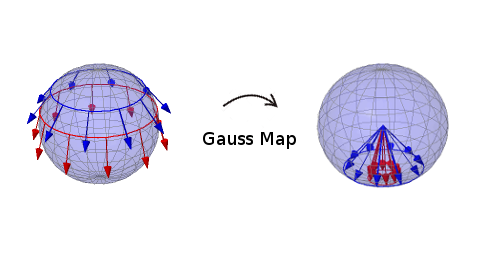
\includegraphics[width=\textwidth]{spherical_gaussmap}

\subsection{Duality between hyperbolic space and de Sitter space} In this section, $\langle \cdot,\cdot\rangle$ denotes the inner product of $\mathbb{R}^{n+1,1}.$
The de Sitter space is the Lorentzian spaceform in the Minkowski space with constant sectional curvature $C=1:$
\eq{\mathbb{S}^{n,1}=\{x\in\mathbb{R}^{n+1,1}: \langle x,x\rangle=1 \},}
whereas the hyperbolic space is a Riemannian spaceform in the Minkowski space with constant sectional curvature $C=-1$:
\eq{\mathbb{H}^{n+1}=\{x\in\mathbb{R}^{n+1,1}: \langle x,x\rangle=-1,~ x^{0}>0\},}
where $x^0$ is the time coordinate.

Similarly, as for the sphere, given an embedding
\eq{x\cn M_0\ra M\sub\H^{n+1}}
of a closed and strictly convex hypersurface, the representation $\~x\in T_x(\R^{n+1,1})$ of the exterior normal vector $\nu\in T_x(\H^{n+1})$ yields the embedding
\eq{\label{HypGaussMap}\~x\cn M_0\ra \~M\sub \S^{n,1}}
of a strictly convex, closed and spacelike hypersurface $\~M.$
We also call this map $\~x$ the {\it{Gauss map of $M$}} and similarly as in the spherical case we have the following theorem:
\Theo{thm}{DeSitterDuality}{\cite[Thm.~10.4.4]{Gerhardt:/2006}
Let $x\cn M\ra \H^{n+1}$ be a closed, connected, strictly convex hypersurface of class $C^{m},$ $m\geq 3,$ then the Gauss map $\~x$ as in \eqref{HypGaussMap} is the embedding of a closed, spacelike, achronal, strictly convex hypersurface $\~M\sub \mathbb{S}^{n,1}$ of class $C^{m-1}.$ Viewing $\~M$ as a codimension $2$ submanifold in $\R^{n+1,1},$ its Gaussian formula is
\eq{\~x_{;ij}=-\~g_{ij}\~x+\~h_{ij}x,}
where $\~g_{ij},$ $\~h_{ij}$ are the metric and the second fundamental form of the hypersurface $\~M\sub \mathbb{S}^{n,1}$ and $x=x(\xi)$ is the embedding of $M$ which also represents the future directed normal vector of $\~M$. The second fundamental form $\~h_{ij}$ is defined with respect to the future directed normal vector, where the time orientation of $N$ is inherited from $\R^{n+1,1}$.

The second fundamental forms of $M,$ $\~M$ and the corresponding principal curvatures $\k_{i},$ $\~\k_{i}$ satisfy
\eq{h_{ij}=\~h_{ij}=\ip{\~x_{;i}}{x_{;j}},\quad \~\k_{i}=\k_{i}^{-1}.}
}
The hypersurface $\tilde{M}$ is called the polar set to $M$ and it can be represented as follows \cite[Thm.~10.4.8]{Gerhardt:/2006}:
$$\tilde{M}=\{y\in \mathbb{S}^{n,1}: \sup_{y\in M}\langle x,y\rangle=0\}.$$
In this model of the hyperbolic space the point $(1,0,\ldots,0)$ is called the {\it{Beltrami point}}. For a given strictly convex hypersurface $M\sub\H^{n+1}$, $M$ bounds a strictly convex body $\hat{M}$ of the hyperbolic space, cf.~\cite[Thm.~10.3.1]{Gerhardt:/2006}, and due to the homogeneity of the hyperbolic space, any point in $\hat{M}$ may act as Beltrami point after suitable ambient change of coordinates. Therefore, in addition to the statement of \cref{DeSitterDuality}, \cite[Thm.~10.4.9.]{Gerhardt:/2006} implies that the dual $\~M$ is contained in the future of the slice $\{x^0=0\}$,
\eq{\~M\sub \S^{n,1}_{+}=\{x\in \S^{n,1}\cn x^0>0\}.}
We will also need the reverse direction starting from a strictly convex, spacelike hypersurface in $\S^{n,1}.$
\Theo{thm}{HyperbolicDuality}{\cite[Thm.~10.4.5]{Gerhardt:/2006}
Let $x\cn \~M\ra \S^{n,1}$ be a closed, connected, spacelike, strictly convex hypersurface of class $C^{m},$ $m\geq 3,$ such that, when viewed as a codimension 2 submanifold in $\R^{n+1,1}$, its Gaussian formula is
\eq{\~x_{;ij}=-\~g_{ij}\~x+\~h_{ij}x,}
where $\~x=\~x(\xi)$ is the embedding, $x$ the future directed normal vector , and $\~g_{ij}$, $\~h_{ij}$ the induced metric and the second fundamental form of the hypersurface in $\S^{n,1}$. Then we define the Gauss map as $x=x(\xi)$
\eq{x\cn \~M\ra \H^{n+1}\sub\R^{n+1,1}.}
The Gauss map is the embedding of a closed, connected, strictly convex hypersurface $M$ in $\H^{n+1}.$
Let $\~g_{ij},$ $\~h_{ij}$ be the metric and the second fundamental form of $M$, then, when viewed as a codimension 2 submanifold, $M$ satisfies the relations
\eq{x_{ij}=g_{ij}x-h_{ij}\~x,}
\eq{h_{ij}=\~h_{ij}=\ip{x_{;i}}{\~x_{;j}},} and
\eq{\~\k_{i}=\k_{i}^{-1},}
where $\k_{i}$, $\~\k_{i}$ are the corresponding principal curvatures.
}
The following illustration shall give a clearer picture of the duality:

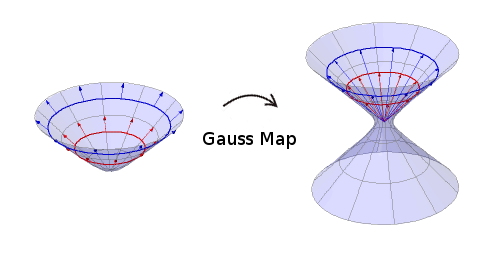
\includegraphics[width=\textwidth]{gaussmap}
\subsection{Dual flows}
We want to deduce the corresponding duality relation for flows of strictly convex hypersurfaces in $\S^{n+1}$, as well as in $\H^{n+1}$ and $\S^{n,1}.$ A similar deduction of these results can be found in \cite[Sec.~4]{Gerhardt:/2015} and \cite{Yu:04/2016}.
For a curvature flow
\eq{\label{NormalFlow}\dot{x}=-\s f\nu,}
where $\s=\ip{\nu}{\nu}$, we want to derive the curvature flow equation of the Gauss maps $\~x$. In both cases the pair $x,\~x$ satisfies
\eq{\ip{x}{\~x}=0,}
where $\ip{\cdot}{\cdot}$ represents the Euclidean and the Minkowski inner product respectively for flows in $\S^{n+1}$ or in $\H^{n+1}$ and $\S^{n,1}$.
Hence
\eq{\ip{\dot{\~x}}{x}=-\ip{\~x}{\dot{x}}=-\ip{\~x}{- \s f\~x}= f.}
 Also, note that $\ip{\~x}{\~x_{;i}}=0$; therefore, due to the Weingarten equation \cite[Lem.~9.2.4, Lem.~10.4.3]{Gerhardt:/2006},
\eq{\ip{\dot{\~x}}{\~x_{;i}}=h^k_i\ip{\dot{\~x}}{x_{;k}}=-h^k_i\ip{\~x}{\dot{x}_{;k}}=h^k_if_{;k}.}
Since $x=\~\nu$ and $\~x_{;i}$ span $T_{\~x}(\S^{n+1})$ and $T_{\~x}(\S^{n,1})$ respectively, we obtain
\eq{\dot{\~x}&=\ip{x}{x} f\~\nu+h^k_mf_{;k}\~g^{ml}\~x_{;l}\\
            &=\~\s f\~\nu+\~b^k_m\~g^{ml}f_{;k}\~x_{;l}\\
            &=\~\s f\~\nu+\~b^{kl}f_{;k}\~x_{;l},}
where $f$ is still evaluated at $\mc{W}$. However, there holds
\eq{\label{DualFlow-3}f(\mc{W})=\fr{1}{f^{-1}(\~{\mc{W}}^{-1})}=\~f^{-1}(\~{\mc{W}})\equiv -\Phi(\~{\mc{W}})}
and hence
\eq{\label{DualHyperbolic}\dot{\~x}=-\~\s\Phi\~\nu-\~b^{kl}\Phi_{;k}\~x_{;l},}
where $\~\s=\ip{\~\nu}{\~\nu}$ and where $\Phi$ is now evaluated at the ``correct" Weingarten map $\~{\mc{W}}$. Hence a flow of the form
\eqref{NormalFlow} in the ambient spaces $\S^{n+1}, \H^{n+1},\S^{n,1}$ has a dual flow of the form \eqref{Flow} in the ambient spaces $\S^{n+1}, \S^{n,1},\H^{n+1}$ respectively.
\section{Locally symmetric spaces}
In this section we prove the Harnack inequalities. We restrict to locally symmetric spaces, since in more general settings we are not aware how to deal with the terms including derivatives of the Riemannian curvature tensor. In order to prove our main theorems, we need the following corollary of \eqref{Ev-u-new} with bonus term $\beta$, which will be the basis for the proofs of all our main theorems.
\Theo{lemma}{Homogeneous}{
Let the ambient space $N$ be locally symmetric, i.e.,
\eq{\-{\n}\overline{\mrm{Rm}}=0.}
Let the speed $f$ satisfy \cref{SpeedAss}, let $\beta\in \R$ and define
\eq{q=t(u-\beta)+\fr{p}{p+1}.}
Then for $p>0$, any strictly convex solution to  \eqref{Flow} satisfies
\eq{\label{Ev-q}\mc{L}q&\geq\fr{t}{\p^{2}}\br{\p''\p+\fr{(1-p)\p'^{2}}{p}}f^{2}+\fr{2t\s}{p}\fr{\p'}{\p}fu+\fr{p+1}{p}(u-\beta)q\\
            &\hp{=}-t\fr{p+1}{p}(u-\beta)^{2}+t\fr{p-1}{p}u^{2}+\fr{2t}{p}\br{u-\fr{df(\L^{\sharp})}{f}}^{2}\\
            &\hp{=}+t\s\br{1-\fr{\operatorname{Tr}_{d_{h}f}h(\cdot,\cdot)}{f}}\overline{\mrm{Rm}}(\dot{x},\nu,\nu,\dot{x})+\fr{2t}{f} \operatorname{Tr}_{d_{h}f}\overline{\mrm{Rm}}(\cdot,\dot{x},\dot{x},\cW(\cdot)),
}
If $p<0$, the inequality is reversed.
}
\pf{
We consider two cases.
\begin{itemize}
  \item  $N=\R^{n+1}$ or $N=\R^{n,1}.$
Recall that the support function is given by $s=\s\ip{x}{\nu}.$
Hence
\eq{\dot{s}=\s\ip{\dot{x}}{\nu}=-\s f}
and
\eq{\ddot{s}&=-\s\dot{f}=\fr{\p'}{\p}f^2-\s df(\dot{\mathcal{W}})=\fr{\p'}{\p}f^2-\s df(A\circ\cW).}
We also have
\eq{\label{R=0-3} u=-\s \fr{\p'}{\p}f+\fr 1f df(\dot{\mathcal{W}})=-\s \fr{\p'}{\p}f+\fr 1f df(A\circ\cW).}
Combining these relations with \cref{InvConc}, in case $p>0$ \eqref{Ev-u} becomes
\eq{\label{R=0-1}
\mathcal{L}u&=\br{\log\p}''\dot{s}^2+\br{\log\p}'\ddot{s}+\frac{\dot{s}}{f}\br{\log\p}'df(\dot{\cW})+\fr 1f d^{2}f(\dot{\cW},\dot{\cW})+\fr 2f \mrm{Tr}_{d_{h}f}h(A(\cdot),A(\cdot))\\
                &\geq \br{\log\p}''\dot{s}^2+\br{\log\p}'\ddot{s}+\frac{\dot{s}}{f}\br{\log\p}'df(\dot{\cW})+\fr{p+1}{p}f^{-2}df(\dot{\mathcal{W}})^{2}\\
                &=\fr{\p''}{\p}f^{2}-\fr{2\s\p'}{\p}df(\dot{\cW})+\fr{p+1}{p}u^{2}+\fr{2(p+1)\s\p'}{p\p}fu+\fr{p+1}{p}\fr{\p'^{2}}{\p^{2}}f^{2}\\
                &=\fr{p+1}{p}u^{2}+\fr{1}{\p^{2}}\br{\p''\p+\fr{(1-p)\p'^{2}}{p}}f^{2}+\fr{2\s}{p}\fr{\p'}{\p}fu,}
with reversed inequality if $p<0$.
\item  $N$ is a space form or as well in the case $f=H.$
                In the case that, we have
\eq{\mrm{Tr}(df\circ (A\circ\L^{\sharp}-\L^{\sharp}\circ A))=0,}
since $\L^{\sharp}$ is a multiple of the identity when $N$ is a space form.


Since $df$ commutes with $\cW$, by \cref{InvConc} we have
\eq{\mrm{Tr}_{d_{h}f}h(A(\cdot),A(\cdot))&=df(\ad(A)\circ\cW\circ A)\\
                        &=df(\ad(\cW\circ A)\circ \cW^{-1}\circ\cW\circ A )\\
                        &\geq \fr 1p f^{-1}df(\cW\circ A)^{2}\\
                        &=\fr{1}{p}f^{-1}df(\dot{\cW}-\L^{\sharp})^{2}\\
                        &=\fr 1p f^{-1}\br{df(\dot{\cW})^{2}-2df(\dot{\cW})df(\L^{\sharp})+df(\L^{\sharp})^{2}}.
                        }
On the other hand, the convexity of $F$ gives
\eq{d^{2}f(\dot{\cW},\dot{\cW})\geq \fr{p-1}{p}f^{-1}df(\dot{\cW})^{2}.}
Consequently, using these last two relations and $u=\fr 1f df(\dot{\mathcal{W}})$, we arrive at
\eq{&\fr 2f\mrm{Tr}_{d_{h}f}h(A(\cdot),A(\cdot))+\fr 1fd^{2}f(\dot{\cW},\dot{\cW})\\
    \geq &~\fr{p+1}{p}f^{-2}df(\dot{\cW})^2-\fr 4pf^{-2} df(\dot{\cW})df(\L^{\sharp})+\fr 2p f^{-2}df(\L^{\sharp})^{2}\\
    =&~\fr{p+1}{p}u^2-\frac{4}{p}\frac{df(\L^{\sharp})}{f}u+\frac{2}{p}\left(\frac{df(\L^{\sharp})}{f}\right)^2}
with reversed inequality if $p<0$.

Therefore, from \eqref{Ev-u} we deduce that if $p>0$, then
\eq{\label{LocHom-1}\mathcal{L}u&\geq \frac{p+1}{p}u^2-\frac{4}{p}\frac{df(\L^{\sharp})}{f}u+\frac{2}{p}\left(\frac{df(\L^{\sharp})}{f}\right)^2
\\
&\hp{=}+\s\br{1-\fr{\operatorname{Tr}_{d_{h}f}h(\cdot,\cdot)}{f}}\overline{\mrm{Rm}}(\dot{x},\nu,\nu,\dot{x})+\fr 2f \operatorname{Tr}_{d_{h}f}\overline{\mrm{Rm}}(\cdot,\dot{x},\dot{x},\cW(\cdot)),
        }
and the inequality is reversed if $p<0$.
\end{itemize}
In all cases we obtain, using \eqref{R=0-1} and \eqref{LocHom-1},
\eq{\mc{L}q&=u-\beta+t\mc{L} u\\
            &=\fr{p+1}{p}(u-\beta)q-t\fr{p+1}{p}(u-\beta)^{2}+t\mc{L}u\\
            &\geq\fr{t}{\p^{2}}\br{\p''\p+\fr{(1-p)\p'^{2}}{p}}f^{2}+\fr{2t\s}{p}\fr{\p'}{\p}fu+\fr{p+1}{p}(u-\beta)q\\
            &\hp{=}-t\fr{p+1}{p}(u-\beta)^{2}+t\fr{p-1}{p}u^{2}+\fr{2t}{p}\br{u-\fr{df(\L^{\sharp})}{f}}^{2}\\
            &\hp{=}+t\s\br{1-\fr{\operatorname{Tr}_{d_{h}f}h(\cdot,\cdot)}{f}}\overline{\mrm{Rm}}(\dot{x},\nu,\nu,\dot{x})+\fr{2t}{f} \operatorname{Tr}_{d_{h}f}\overline{\mrm{Rm}}(\cdot,\dot{x},\dot{x},\cW(\cdot)),
}
with reversed inequality of $p<0$.
}
Having established the previous lemma, we can now prove various Harnack inequalities. We proceed from the most general ambient space to the specific ones.
\subsection*{Euclidean and Minkowski space}
%\section{Euclidean and Minkowski space}
In the case that the ambient curvature vanishes, we obtain the following Harnack inequalities for anisotropic flows claimed in Theorem \ref{Euclidean}. In particular, the theorem includes and extend the well-known Harnack inequalities from \cite{Andrews:09/1994} in the Euclidean space and they are completely new in the Minkowski space.
\Theo{thm}{R=0}{
Let $N$ be either the Euclidean or the Minkowski space and let $F$, $\p$ and $\psi$ satisfy the assumptions of \cref{Euclidean}. Then along \eqref{Flow}, if $p>0$ there holds
\eq{tu+\fr{p}{p+1}\geq 0}
and if $p<0$ the inequality is reversed.
}
\pf{Apply \eqref{Ev-q} with $\beta=0$ to obtain that $q$ satisfies
\eq{\mc{L}q\geq \fr{2\s}{p}\fr{\p'}{\p}fq-\fr{2\s}{p+1}\fr{\p'}{\p}f+\fr{p+1}{p}uq}
with reversed inequality if $p<0$. If the ambient space is Euclidean, the maximum principle gives the Harnack estimate. If $N=\mathbb{R}^{n,1}$, due to our assumptions in Theorem \ref{Euclidean}, we can apply the maximum principle on the compact set $K$ and prove the claimed Harnack inequalities in each case.
}
\subsection*{Locally symmetric Einstein spaces of non-negative sectional curvature}
Here we obtain Harnack inequalities for the mean curvature flow:
\Theo{thm}{LocSymm}{
Suppose $N$ is a Riemannian locally symmetric Einstein space with non-negative sectional curvature. Let $f=H$. Then for any strictly convex solution to \eqref{Flow} there holds
\eq{\label{Bonus}t\br{u-\fr{\-R}{n+1}}+\fr{1}{2}\geq 0,}
where $\-R$ is the scalar curvature.
}
\pf{
We use \eqref{Ev-q} with
$\beta=\fr{\-R}{n+1},$
where $R$ is the scalar curvature. In this situation we have $\s=1$ and $df(\cW)=H$ and hence the last line of \eqref{Ev-q} is non-negative. Furthermore there holds
\eq{df(\L^{\sharp})=-\mrm{Tr}(\overline{\mrm{Rm}}(\cdot,\dot{x},\nu,\cdot))=-\overline{\mrm{Rc}}(\dot{x},\nu)=\fr{\-R}{n+1}f.}
Hence the claim follows from the maximum principle applied to \eqref{Ev-q}.
}
\subsection*{The sphere}
In the case of the sphere, inequality \eqref{Bonus} is precisely the Harnack inequality with bonus term as it was already deduced in \cite{BryanIvaki:08/2015}.
We recover the class of speeds for which we could prove a Harnack inequality without bonus term in \cite{BIS1}.
\Theo{thm}{Sphere}{
Suppose $N=\S^{n+1}$ and $F$ is a monotone, convex and $1$-homogeneous curvature function. Let $0<p\leq 1$ and $f=F^p.$ Then for any strictly convex solution to \eqref{Flow} there holds
\eq{tu+\fr{p}{p+1}\geq 0.}
}
\pf{
The last line of \eqref{Ev-q} is non-negative. Also note that
$\L=fg.$
We calculate
\eq{\nonumber-t\fr{p+1}{p}u^{2}+t\fr{p-1}{p}u^{2}+\fr{2t}{p}\br{u-\fr{df(\L^{\sharp})}{f}}^{2}
&=-\fr{4t}{p}u\fr{df(\L^{\sharp})}{f}+\fr{2t}{p}\br{\fr{df(\L^{\sharp})}{f}}^{2}\\
&\geq -\fr{4}{p}q\fr{df(\L^{\sharp})}{f}+\fr{4}{p+1}\fr{df(\L^{\sharp})}{f},
    }
and hence the maximum principle implies the claim again.
}
By applying the dual flow method developed in \Cref{Duality}, we obtain pseudo-Harnack inequalities
for a class of inverse curvature flows.
 \Theo{thm}{ExpandingSphere}{
Suppose $N=\S^{n+1}$ and $F$ is a monotone, inverse convex and $1$-homogeneous curvature function. Let $-1\leq p<0$ and $f=-F^{p}.$ Then for any strictly convex solution of \eqref{NormalFlow} we have
\eq{\del_t\br{ft^{\fr{p}{p-1}}}\leq 0.}
}
\pf{
The dual flow of \eqref{DualHyperbolic} with speed
\eq{\Phi(\~{\mc{W}})=-f(\mc{W})=-\mrm{sgn}(p)F^{p}(\mc{W})=\~F^{-p}(\~{\mc{W}})}
satisfies the assumptions of \cref{Sphere}, which in particular implies
\eq{\del_t\br{\Phi t^{\fr{-p}{-p+1}}}\geq 0.}
}
\subsection*{De Sitter space}
For flows of spacelike hypersurfaces in Lorentzian manifolds of nonvanishing curvature, the second line of \eqref{Ev-q} can behave rather differently, since $\nu$ is timelike. Hence, in the de Sitter space of constant sectional curvature $K_{N}=1$ we obtain a similar result as in the sphere, but only for flow with principal curvatures bounded be $1$. This is equivalent to convexity by horospheres for the dual hypersurfaces in the hyperbolic space and hence seems to be a natural assumption for flows in the de Sitter space.
\Theo{thm}{DeSitter}{
Let $N=\mathbb{S}^{n,1}$ and $F$ be a monotone, convex and $1$-homogeneous curvature function. Let $0<p\leq 1$ and set $f=F^p$. Then for any solution $x$ of \eqref{Flow} that the condition $0<\kappa_i\leq 1$ is always satisfied on $[0,T^{\ast})$ there holds
\eq{tu+\fr{p}{p+1}\geq 0.}
}
\pf{
Recall that $-V=\dot{x}+\sigma f\nu.$ We start with the following observations:
\begin{align*}
\overline{\mrm{Rm}}(\dot{x},\nu,\nu,\dot{x})&=-\langle \dot{x},\dot{x}\rangle-\langle \dot{x},\nu\rangle^2\\
&=f^2-\langle V,V\rangle-f^2\leq 0,
\end{align*}
since $V$ is spacelike, and
\begin{align*}
\mrm{Tr}_{d_{h}f}\overline{\mrm{Rm}}(\cdot,\dot{x},\dot{x},\cW(\cdot))&=\mrm{Tr}_{d_{h}f}\br{\-g(\dot{x},\dot{x})g(\cdot,\cW(\cdot))-\-g(\cdot,\dot{x})\-g(\dot{x},\cW(\cdot))}\\
&=\mrm{Tr}_{d_{h}f\ast\cW}\br{-f^{2}g+g(V,V)g-g(\cdot,V)g(\cdot,V)}\\
&\geq -f^{2}df(\cW).
\end{align*}

The identity \eqref{Ev-q} with $\beta=0$, these last two inequalities
imply that
\eq{\label{xx}\mathcal{L}q&\geq\br{\fr{p+1}{p}u-\fr{4}{p}\fr{df(\L^{\sharp})}{f}}q+\fr{2t}{p}\left(\br{\fr{df(\L^{\sharp})}{f}}^2-(df(\cW))^{2}\right)\\
            &\hp{=}+\fr{4}{p+1}\fr{df(\L^{\sharp})}{f}.}
In addition, since $0<\kappa_i\leq 1$ and $\L^{\sharp}=f\operatorname{Id}$, the monotonicity of $f$ gives
\[pf=df(\cW)\leq df(\operatorname{Id}).\]
The result now follows from the maximum principle.
}
\Theo{rem}{}{
In the de Sitter space, we cannot expect to obtain a Harnack estimate with a bonus term for mean curvature flow as in the spherical case. To see that, we will look at ancient solutions with $0<\kappa_i\leq 1$ to the mean curvature flow.

The evolution equation of $H$ is given by
\[\partial_tH=\Delta H+T\ast\nabla H-|A|^2H+nH.\]
If there was a Harnack inequality for mean curvature flow of the following form
\[\partial_tH-nH+\frac{H}{2t}\geq 0,\]
then for an ancient solution we would have
$\partial_tH-nH\geq 0.$
So evolution equation of $H$ would yield
$\Delta H+T\ast\nabla H-|A|^2H\geq 0;$ therefore, $H(\cdot,t)=0.$
}
%\Theo{thm}{MCF with bonus}{Let $N=\mathbb{S}^{n,1}$ and $f=H$. Then under \eqref{Flow} we have
%\[\partial_tH-nH+\frac{H}{2t}\geq 0.\]}
%\pf{Define $q:=w-nt$. Using (\ref{xx}) and ignoring its last two terms (since their sum is non-negative), we deduce that for $f=H:$
%\[\dot{q}\geq \Delta {q}+T\ast\n q+2\left(u-n\right)q.\]
%Hence by the maximum principle, $q$ remains positive. This implies that
%\[\partial_t H-nH+\frac{H}{2t}\geq 0.\]
%}

With precisely the same proof as for \cref{Sphere}, we obtain, using \eqref{DualHyperbolic} and \cref{DeSitter}, the following pseudo-Harnack inequality for expanding flows of the hyperbolic space, which is to our knowledge the first such inequality for hypersurface flows in the hyperbolic space:
\Theo{thm}{Hyperbolic}{Let $N=\H^{n+1}$ and $F$ be a monotone, 1-homogeneous and inverse convex curvature function. If $-1\leq p<0$, then any horoconvex solution to \eqref{NormalFlow} with speed $f=-F^{p}$
satisfies
\[\del_t\br{ft^{\fr{p}{p-1}}}\leq 0.\]
}
\pf{The speed of the dual flow \eqref{DualHyperbolic} is
\[\Phi(\~{\mc{W}})=-f(\mc{W})=-\mrm{sgn}(p)F^p(\mc{W})=-\mrm{sgn}(p)F^p(\~{\mc{W}}^{-1})=-\mrm{sgn}(p)\fr{1}{\~F^p(\~{\mc{W}})}\]
and if $-1\leq p<0$, then
\[\Phi(\~{\mc{W}})=\mrm{sgn}(-p)\~F^{-p}(\~{\mc{W}}).\]
Thus for $-1\leq p<0,$ the assumptions of \cref{DeSitter} are satisfied with $0<-p\leq 1$; therefore,
\[\del_t\br{\Phi t^{\fr{-p}{-p+1}}}\geq 0\Rightarrow \del_t\br{f t^{\fr{p}{p-1}}}\leq 0.\]
}
\section{Preserving convexity/horoconvexity}
In our main theorems we always assume that we have a strictly convex flow, in fact, otherwise we can not even write down the reparametrization \eqref{Flow}. In this section we justify this assumption by showing that in many cases the strict convexity of the flow hypersurfaces is preserved under \eqref{Flow}. We start with the de Sitter space.
\Theo{prop}{PresConvDeSitter}{
Let $N=\S^{n,1}$ and $F$ be a monotone, convex and $1$-homogeneous. Let $0<p\leq 1$ and set $f=F^p$. Let $M_0\sub N$ be a strictly convex, closed and spacelike hypersurface, such that the Beltrami point of the dual hypersurface $\~M_0$ lies in the interior of the convex body enclosed by $\~M_0$. Then the strict convexity is preserved under the flow
\eq{\label{PresConvDeSitter-1}\dot{x}=f\nu.}
}
\pf{
We use the dual inverse curvature flow in the hyperbolic space $\H^{n+1}$. Using \Cref{gauss_duality} we obtain that up to reparametrization the dual flow, denoted by $\~x$ evolves according to
\eq{\label{PresConvDeSitter-2}\dot{\~x}=\fr{1}{\~F^p}\~\nu,\quad 0<p\leq 1,}
where $\~\nu$ is the outward unit normal to the flow hypersurfaces in $\H^{n+1}$. Now $\~M_0$ is starshaped with respect to the origin in $\H^{n+1}$ (the Beltrami point) and $\~F$ is the inverse of $F$. Hence $\~F$ is concave, compare \Cref{subsec:bg_speed}. Precisely under these assumptions on $\~F$ and $p$ we have shown in \cite[Thm.~1.2]{Scheuer:05/2015}, that the flow \eqref{PresConvDeSitter-2} with initial hypersurface $\~M_0$ exists for all times (regardless of preserved convexity!).
Hence, at a first time $t_0<\8$ where \eqref{PresConvDeSitter-1} loses convexity, the principal curvatures of $\~M_{t_0}$ are still bounded, which is a contradiction,\footnote{$M_0$ is strictly convex $\Rightarrow\~M_0$ is strictly convex $\Rightarrow\~M_0$ is starshaped (see, e.g., \cite[Section 3.2]{Gerhardt:/2006} for the last step)  $\Rightarrow\~\kappa_i\leq c_{\tilde{M}_0},~\forall t>0$  $\Rightarrow\kappa_i$ cannot go to zero as $t$ approaches $t_0$} so such a time $t_0$ does not exist.
}

To show that the condition $\k_i\leq 1$ is preserved we need an additional assumption on the speed, namely that $f=F^p$ is also concave.
Then we get:
\Theo{thm}{PresCurv}{
Let $N=\S^{n,1}$ and $F$ be a monotone, convex and $1$-homogeneous. Let $0<p\leq 1$, set $f=F^p$ and suppose that $f$ is concave. Let $M_0\sub N$ be a strictly convex, closed and spacelike hypersurface, such that $\k_i\leq 1$ for $1\leq i\leq n$ and the Beltrami point of the dual hypersurface $\~M_0$ lies in the interior of the convex body enclosed by $\~M_0$. Then the condition $\k_i\leq 1$ is preserved under the flow
\eq{\label{PresCurv-1}\dot{x}=f\nu.}
}
\pf{
Due to \cite[Lemma~2.3.1, Lemma~2.4.3]{Gerhardt:/2006}, along \eqref{PresCurv-1} the tensor
\eq{S_{ij}=h_{ij}-g_{ij}}
satisfies the evolution equation
\eq{\dot{S}_{ij}-f^{kl}S_{ij;kl}=&-f^{kl}h_{kr}h^r_lh_{ij}+(1+p)f(h^k_ih_{kj}+g_{ij})-f^{kl}g_{kl}h_{ij}-2fh_{ij}\\
    &+f^{kl,rs}h_{kl;i}h_{rs;j}\\
                        \equiv& N_{ij}.
}
We use Hamilton's tensor maximum principle, \cite[Thm.~9.1]{Hamilton:/1982}. At a unit null eigenvector $v$ of $S_{ij}$ we obtain, also using the concavity of $f$,
\eq{N_{ij}v^iv^j&\leq -f^{kl}h_{kr}h^r_l+2f+2pf-f^{kl}g_{kl}-2f\\
                &=-f^{kl}(h_{kr}h^r_l-2h_{kl}+g_{kl})\\
                &\leq 0.}
Hence \cite[Thm.~9.1]{Hamilton:/1982} is applicable and we conclude that $S_{ij}$ remains non-positive.
}
\section{Cross curvature flow}\label{cross}
Let $(M^3,g)$ be a Riemannian 3-manifold with negative sectional curvature. The cross curvature tensor is defined by
\[c_{ij}:=(E^{-1})_{ij}\det E=\frac{1}{2}\mu^{ipq}\mu^{jrs}E_{pr}E_{qs}=\frac{1}{8}\mu^{pqk}\mu^{rsl}R_{ilpq}R_{kjrs},\]
where $E_{ij}:=R_{ij}-\frac{1}{2}Rg_{ij}$ is the Einstein tensor, $R_{ijkl}$ is the Riemann curvature tensor, $R_{ij}$ is the Ricci curvature tensor and $R$ is the scalar curvature, $\det E:=\det E_{ij}/\det g_{ij}$ and $\mu^{ijk}$ are the component of the volume form.

A one-parameter family of 3-manifolds $(M,g(t))$ with negative sectional curvature is a solution of the XCF if
\[\partial_tg_{ij}=2c_{ij}.\]
Now suppose metrics are locally isometrically embeddable in Minkowski space $\mathbb{R}^{3,1}$. The following observation is due to Andrews, which recently appeared in \cite{AndrewsChenFangMcCoy:/2015}.

Recall that the Gauss equation in $\mathbb{R}^{3,1}$ reads
\[
R_{ijkl} = -(h_{ik}h_{jl} - h_{il}h_{jk}).
\]
Tracing with respect to $g^{ik}$ gives
\[
R_{jl} = -(Hh_{jl} - h^k_lh_{jk}), \quad R = -(H^2 - |A|^2),
\]
where $|A|^2=g^{ik}g^{jl}h_{ij}h_{kl}.$
Thus we have
\[
E_{ij} = H\left(\frac{H}{2}g_{ij} - h_{ij}\right) + \left(h^k_ih_{kj} - \frac{1}{2}|A|^2g_{ij}\right).
\]
In an orthonormal frame which diagonalizes the second fundamental form, we get for $i=1$:
\[
\begin{split}
E_{11} &= \frac{1}{2}\left(H^2 - |A|^2\right) + h^1_1 h_{11} - Hh_{11} \\
&= \frac{1}{2}\left(2(h_{11}h_{22} + h_{11}h_{33} + h_{22}h_{33})\right) + h_{11}^2 - \left(h_{11} + h_{22} + h_{33}\right) h_{11} \\
&= h_{22}h_{33},
\end{split}
\]
and similarly for $i=2,3$. That is,
\[
E = \begin{pmatrix}
\kappa_2 \kappa_3 & 0 & 0 \\
0 & \kappa_1\kappa_3 & 0 \\
0 & 0 & \kappa_1\kappa_2
\end{pmatrix}
\]
where $\kappa_i$ denote the principal curvatures. In particular, $\det E = K^2,$ where $K$ is the Gauss curvature. If $M$ is strictly convex, then $E$ is positive definite, hence invertible. In this case, the cross curvature tensor is
\[
c_{ij} = ({\det} E) (E^{-1})_{ij} = \begin{pmatrix}
\kappa_1^2 \kappa_2 \kappa_3 & 0 & 0 \\
0 & \kappa_1\kappa_2^2 \kappa_3 & 0 \\
0 & 0 & \kappa_1\kappa_2\kappa_3^2
\end{pmatrix} = Kh_{ij}.
\]
Now the uniqueness result of Buckland \cite{Buckland:/2006} shows that $(M,g(t))$ is a solution of (\ref{FlowStandard}) with $N=\mathbb{R}^{3,1}$, $f=K$.

The Harnack inequality for the cross curvature flow for metrics that are locally isometrically embeddable in Minkowski space $\mathbb{R}^{3,1}$ now follows from \Cref{Euclidean}:
\begin{align}\label{cross harnack}
\partial_t \sqrt{{\det} E} - \frac{1}{\sqrt{{\det}E}}E^{ij} \nabla_i \left(\sqrt{{\det}E}\right) \nabla_j \left(\sqrt{{\det}E}\right) + \frac{3}{4 t} \sqrt{{\det}E} \geq 0.
\end{align}


\bibliographystyle{amsplain}
\bibliography{Bibliography}


\end{document}

